%**************************************%
%* Generated from MathBook XML source *%
%*    on 2016-08-14T15:38:59-04:00    *%
%*                                    *%
%*   http://mathbook.pugetsound.edu   *%
%*                                    *%
%**************************************%
\documentclass[10pt,]{book}
%% Load geometry package to allow page margin adjustments
\usepackage{geometry}
\geometry{letterpaper,total={5.0in,9.0in}}
%% Custom Preamble Entries, early (use latex.preamble.early)
%% Inline math delimiters, \(, \), need to be robust
%% 2016-01-31:  latexrelease.sty  supersedes  fixltx2e.sty
%% If  latexrelease.sty  exists, bugfix is in kernel
%% If not, bugfix is in  fixltx2e.sty
%% See:  https://tug.org/TUGboat/tb36-3/tb114ltnews22.pdf
%% and read "Fewer fragile commands" in distribution's  latexchanges.pdf
\IfFileExists{latexrelease.sty}{}{\usepackage{fixltx2e}}
%% Page Layout Adjustments (latex.geometry)
%% This LaTeX file may be compiled with pdflatex, xelatex, or lualatex
%% The following provides engine-specific capabilities
%% Generally, xelatex and lualatex will do better languages other than US English
%% You can pick from the conditional if you will only ever use one engine
\usepackage{ifthen}
\usepackage{ifxetex,ifluatex}
\ifthenelse{\boolean{xetex} \or \boolean{luatex}}{%
%% begin: xelatex and lualatex-specific configuration
%% fontspec package will make Latin Modern (lmodern) the default font
\ifxetex\usepackage{xltxtra}\fi
\usepackage{fontspec}
%% realscripts is the only part of xltxtra relevant to lualatex 
\ifluatex\usepackage{realscripts}\fi
%% 
%% Extensive support for other languages
\usepackage{polyglossia}
\setdefaultlanguage{english}
%% Magyar (Hungarian)
\setotherlanguage{magyar}
%% Spanish
\setotherlanguage{spanish}
%% Vietnamese
\setotherlanguage{vietnamese}
%% end: xelatex and lualatex-specific configuration
}{%
%% begin: pdflatex-specific configuration
%% translate common Unicode to their LaTeX equivalents
%% Also, fontenc with T1 makes CM-Super the default font
%% (\input{ix-utf8enc.dfu} from the "inputenx" package is possible addition (broken?)
\usepackage[T1]{fontenc}
\usepackage[utf8]{inputenc}
%% end: pdflatex-specific configuration
}
%% Monospace font: Inconsolata (zi4)
%% Sponsored by TUG: http://levien.com/type/myfonts/inconsolata.html
%% See package documentation for excellent instructions
%% One caveat, seem to need full file name to locate OTF files
%% Loads the "upquote" package as needed, so we don't have to
%% Upright quotes might come from the  textcomp  package, which we also use
%% We employ the shapely \ell to match Google Font version
%% pdflatex: "varqu" option produces best upright quotes
%% xelatex,lualatex: add StylisticSet 1 for shapely \ell
%% xelatex,lualatex: add StylisticSet 2 for plain zero
%% xelatex,lualatex: we add StylisticSet 3 for upright quotes
%% 
\ifthenelse{\boolean{xetex} \or \boolean{luatex}}{%
%% begin: xelatex and lualatex-specific monospace font
\usepackage{zi4}
\setmonofont[BoldFont=Inconsolatazi4-Bold.otf,StylisticSet={1,3}]{Inconsolatazi4-Regular.otf}
%% end: xelatex and lualatex-specific monospace font
}{%
%% begin: pdflatex-specific monospace font
\usepackage[varqu]{zi4}
%% end: pdflatex-specific monospace font
}
%% Symbols, align environment, bracket-matrix
\usepackage{amsmath}
\usepackage{amssymb}
%% allow more columns to a matrix
%% can make this even bigger by overriding with  latex.preamble.late  processing option
\setcounter{MaxMatrixCols}{30}
%%
%% Color support, xcolor package
%% Always loaded.  Used for:
%% mdframed boxes, add/delete text, author tools
\PassOptionsToPackage{usenames,dvipsnames,svgnames,table}{xcolor}
\usepackage{xcolor}
%%
%% Semantic Macros
%% To preserve meaning in a LaTeX file
%% Only defined here if required in this document
%% Used for inline definitions of terms
\newcommand{\terminology}[1]{\textbf{#1}}
%% Subdivision Numbering, Chapters, Sections, Subsections, etc
%% Subdivision numbers may be turned off at some level ("depth")
%% A section *always* has depth 1, contrary to us counting from the document root
%% The latex default is 3.  If a larger number is present here, then
%% removing this command may make some cross-references ambiguous
%% The precursor variable $numbering-maxlevel is checked for consistency in the common XSL file
\setcounter{secnumdepth}{3}
%% Environments with amsthm package
%% Theorem-like environments in "plain" style, with or without proof
\usepackage{amsthm}
\theoremstyle{plain}
%% Numbering for Theorems, Conjectures, Examples, Figures, etc
%% Controlled by  numbering.theorems.level  processing parameter
%% Always need a theorem environment to set base numbering scheme
%% even if document has no theorems (but has other environments)
\newtheorem{theorem}{Theorem}[section]
%% Only variants actually used in document appear here
%% Style is like a theorem, and for statements without proofs
%% Numbering: all theorem-like numbered consecutively
%% i.e. Corollary 4.3 follows Theorem 4.2
\newtheorem{algorithm}[theorem]{Algorithm}
%% Definition-like environments, normal text
%% Numbering is in sync with theorems, etc
\theoremstyle{definition}
\newtheorem{definition}[theorem]{Definition}
%% Remark-like environments, normal text
%% Numbering is in sync with theorems, etc
\theoremstyle{definition}
\newtheorem{note}[theorem]{Note}
\newtheorem{observation}[theorem]{Observation}
%% Example-like environments, normal text
%% Numbering is in sync with theorems, etc
\theoremstyle{definition}
\newtheorem{example}[theorem]{Example}
%% Miscellaneous environments, normal text
%% Numbering for inline exercises and lists is in sync with theorems, etc
\theoremstyle{definition}
\newtheorem{exercise}[theorem]{Exercise}
%% Localize LaTeX supplied names (possibly none)
\renewcommand*{\proofname}{Proof}
\renewcommand*{\chaptername}{Chapter}
%% Equation Numbering
%% Controlled by  numbering.equations.level  processing parameter
\numberwithin{equation}{section}
%% For improved tables
\usepackage{array}
%% Some extra height on each row is desirable, especially with horizontal rules
%% Increment determined experimentally
\setlength{\extrarowheight}{0.2ex}
%% Define variable thickness horizontal rules, full and partial
%% Thicknesses are 0.03, 0.05, 0.08 in the  booktabs  package
\makeatletter
\newcommand{\hrulethin}  {\noalign{\hrule height 0.04em}}
\newcommand{\hrulemedium}{\noalign{\hrule height 0.07em}}
\newcommand{\hrulethick} {\noalign{\hrule height 0.11em}}
%% We preserve a copy of the \setlength package before other
%% packages (extpfeil) get a chance to load packages that redefine it
\let\oldsetlength\setlength
\newlength{\Oldarrayrulewidth}
\newcommand{\crulethin}[1]%
{\noalign{\global\oldsetlength{\Oldarrayrulewidth}{\arrayrulewidth}}%
\noalign{\global\oldsetlength{\arrayrulewidth}{0.04em}}\cline{#1}%
\noalign{\global\oldsetlength{\arrayrulewidth}{\Oldarrayrulewidth}}}%
\newcommand{\crulemedium}[1]%
{\noalign{\global\oldsetlength{\Oldarrayrulewidth}{\arrayrulewidth}}%
\noalign{\global\oldsetlength{\arrayrulewidth}{0.07em}}\cline{#1}%
\noalign{\global\oldsetlength{\arrayrulewidth}{\Oldarrayrulewidth}}}
\newcommand{\crulethick}[1]%
{\noalign{\global\oldsetlength{\Oldarrayrulewidth}{\arrayrulewidth}}%
\noalign{\global\oldsetlength{\arrayrulewidth}{0.11em}}\cline{#1}%
\noalign{\global\oldsetlength{\arrayrulewidth}{\Oldarrayrulewidth}}}
%% Single letter column specifiers defined via array package
\newcolumntype{A}{!{\vrule width 0.04em}}
\newcolumntype{B}{!{\vrule width 0.07em}}
\newcolumntype{C}{!{\vrule width 0.11em}}
\makeatother
%% Figures, Tables, Listings, Floats
%% The [H]ere option of the float package fixes floats in-place,
%% in deference to web usage, where floats are totally irrelevant
%% We re/define the figure, table and listing environments, if used
%%   1) New mbxfigure and/or mbxtable environments are defined with float package
%%   2) Standard LaTeX environments redefined to use new environments
%%   3) Standard LaTeX environments redefined to step theorem counter
%%   4) Counter for new environments is set to the theorem counter before caption
%% You can remove all this figure/table setup, to restore standard LaTeX behavior
%% HOWEVER, numbering of figures/tables AND theorems/examples/remarks, etc
%% WILL ALL de-synchronize with the numbering in the HTML version
%% You can remove the [H] argument of the \newfloat command, to allow flotation and 
%% preserve numbering, BUT the numbering may then appear "out-of-order"
\usepackage{float}
\usepackage[bf]{caption} % http://tex.stackexchange.com/questions/95631/defining-a-new-type-of-floating-environment 
\usepackage{newfloat}
% Figure environment setup so that it no longer floats
\SetupFloatingEnvironment{figure}{fileext=lof,placement={H},within=section,name=Figure}
% figures have the same number as theorems: http://tex.stackexchange.com/questions/16195/how-to-make-equations-figures-and-theorems-use-the-same-numbering-scheme 
\makeatletter
\let\c@figure\c@theorem
\makeatother
% Table environment setup so that it no longer floats
\SetupFloatingEnvironment{table}{fileext=lot,placement={H},within=section,name=Table}
% tables have the same number as theorems: http://tex.stackexchange.com/questions/16195/how-to-make-equations-figures-and-theorems-use-the-same-numbering-scheme 
\makeatletter
\let\c@table\c@theorem
\makeatother
%% Raster graphics inclusion, wrapped figures in paragraphs
%% \resizebox sometimes used for images in side-by-side layout
\usepackage{graphicx}
%%
%% Program listing support, for inline code, Sage code
\usepackage{listings}
%% We define the listings font style to be the default "ttfamily"
%% To fix hyphens/dashes rendered in PDF as fancy minus signs by listing
%% http://tex.stackexchange.com/questions/33185/listings-package-changes-hyphens-to-minus-signs
\makeatletter
\lst@CCPutMacro\lst@ProcessOther {"2D}{\lst@ttfamily{-{}}{-{}}}
\@empty\z@\@empty
\makeatother
\ifthenelse{\boolean{xetex}}{}{%
%% begin: pdflatex-specific listings configuration
%% translate U+0080 - U+00F0 to their textmode LaTeX equivalents
%% Data originally from https://www.w3.org/Math/characters/unicode.xml, 2016-07-23
%% Lines marked in XSL with "$" were converted from mathmode to textmode
\lstset{extendedchars=true}
\lstset{literate={ }{{~}}{1}{¡}{{\textexclamdown }}{1}{¢}{{\textcent }}{1}{£}{{\textsterling }}{1}{¤}{{\textcurrency }}{1}{¥}{{\textyen }}{1}{¦}{{\textbrokenbar }}{1}{§}{{\textsection }}{1}{¨}{{\textasciidieresis }}{1}{©}{{\textcopyright }}{1}{ª}{{\textordfeminine }}{1}{«}{{\guillemotleft }}{1}{¬}{{\textlnot }}{1}{­}{{\-}}{1}{®}{{\textregistered }}{1}{¯}{{\textasciimacron }}{1}{°}{{\textdegree }}{1}{±}{{\textpm }}{1}{²}{{\texttwosuperior }}{1}{³}{{\textthreesuperior }}{1}{´}{{\textasciiacute }}{1}{µ}{{\textmu }}{1}{¶}{{\textparagraph }}{1}{·}{{\textperiodcentered }}{1}{¸}{{\c{}}}{1}{¹}{{\textonesuperior }}{1}{º}{{\textordmasculine }}{1}{»}{{\guillemotright }}{1}{¼}{{\textonequarter }}{1}{½}{{\textonehalf }}{1}{¾}{{\textthreequarters }}{1}{¿}{{\textquestiondown }}{1}{À}{{\`{A}}}{1}{Á}{{\'{A}}}{1}{Â}{{\^{A}}}{1}{Ã}{{\~{A}}}{1}{Ä}{{\"{A}}}{1}{Å}{{\AA }}{1}{Æ}{{\AE }}{1}{Ç}{{\c{C}}}{1}{È}{{\`{E}}}{1}{É}{{\'{E}}}{1}{Ê}{{\^{E}}}{1}{Ë}{{\"{E}}}{1}{Ì}{{\`{I}}}{1}{Í}{{\'{I}}}{1}{Î}{{\^{I}}}{1}{Ï}{{\"{I}}}{1}{Ð}{{\DH }}{1}{Ñ}{{\~{N}}}{1}{Ò}{{\`{O}}}{1}{Ó}{{\'{O}}}{1}{Ô}{{\^{O}}}{1}{Õ}{{\~{O}}}{1}{Ö}{{\"{O}}}{1}{×}{{\texttimes }}{1}{Ø}{{\O }}{1}{Ù}{{\`{U}}}{1}{Ú}{{\'{U}}}{1}{Û}{{\^{U}}}{1}{Ü}{{\"{U}}}{1}{Ý}{{\'{Y}}}{1}{Þ}{{\TH }}{1}{ß}{{\ss }}{1}{à}{{\`{a}}}{1}{á}{{\'{a}}}{1}{â}{{\^{a}}}{1}{ã}{{\~{a}}}{1}{ä}{{\"{a}}}{1}{å}{{\aa }}{1}{æ}{{\ae }}{1}{ç}{{\c{c}}}{1}{è}{{\`{e}}}{1}{é}{{\'{e}}}{1}{ê}{{\^{e}}}{1}{ë}{{\"{e}}}{1}{ì}{{\`{\i}}}{1}{í}{{\'{\i}}}{1}{î}{{\^{\i}}}{1}{ï}{{\"{\i}}}{1}{ð}{{\dh }}{1}{ñ}{{\~{n}}}{1}{ò}{{\`{o}}}{1}{ó}{{\'{o}}}{1}{ô}{{\^{o}}}{1}{õ}{{\~{o}}}{1}{ö}{{\"{o}}}{1}{÷}{{\textdiv }}{1}{ø}{{\o }}{1}{ù}{{\`{u}}}{1}{ú}{{\'{u}}}{1}{û}{{\^{u}}}{1}{ü}{{\"{u}}}{1}{ý}{{\'{y}}}{1}{þ}{{\th }}{1}{ÿ}{{\"{y}}}{1}}
%% end: pdflatex-specific listings configuration
}
%% End of generic listing adjustments
%% Generic input, listings package: boxed, white, line breaking, language per instance
%% Colors match a subset of Google prettify "Default" style
%% Set latex.print='yes" to get all black
%% http://code.google.com/p/google-code-prettify/source/browse/trunk/src/prettify.css
\definecolor{identifiers}{rgb}{0.375,0,0.375}
\definecolor{comments}{rgb}{0.5,0,0}
\definecolor{strings}{rgb}{0,0.5,0}
\definecolor{keywords}{rgb}{0,0,0.5}
\lstdefinestyle{genericinput}{breaklines=true,breakatwhitespace=true,columns=fixed,frame=single,xleftmargin=4ex,xrightmargin=4ex,
basicstyle=\small\ttfamily,identifierstyle=\color{identifiers},commentstyle=\color{comments},stringstyle=\color{strings},keywordstyle=\color{keywords}}
%% Multiple column, column-major lists
\usepackage{multicol}
%% More flexible list management, esp. for references and exercises
%% But also for specifying labels (i.e. custom order) on nested lists
\usepackage{enumitem}
%% Lists of references in their own section, maximum depth 1
\newlist{referencelist}{description}{4}
\setlist[referencelist]{leftmargin=!,labelwidth=!,labelsep=0ex,itemsep=1.0ex,topsep=1.0ex,partopsep=0pt,parsep=0pt}
%% Lists of exercises in their own section, maximum depth 4
\newlist{exerciselist}{description}{4}
\setlist[exerciselist]{leftmargin=0pt,itemsep=1.0ex,topsep=1.0ex,partopsep=0pt,parsep=0pt}
%% Indented groups of exercises within an exercise section, maximum depth 4
\newlist{exercisegroup}{description}{4}
\setlist[exercisegroup]{leftmargin=2em,labelindent=2em,itemsep=1.0ex,topsep=1.0ex,partopsep=0pt,parsep=0pt}
%% Support for index creation
%% imakeidx package does not require extra pass (as with makeidx)
%% We set the title of the "Index" section via a keyword
%% And we provide language support for the "see" phrase
\usepackage{imakeidx}
\makeindex[title=Index, intoc=true]
\renewcommand{\seename}{see}
%% Package for tables spanning several pages
\usepackage{longtable}
%% hyperref driver does not need to be specified
\usepackage{hyperref}
%% configure hyperref's  \url  to match listings' inline verbatim
\renewcommand\UrlFont{\small\ttfamily}
%% Hyperlinking active in PDFs, all links solid and blue
\hypersetup{colorlinks=true,linkcolor=blue,citecolor=blue,filecolor=blue,urlcolor=blue}
\hypersetup{pdftitle={Applied Discrete Structures}}
%% If you manually remove hyperref, leave in this next command
\providecommand\phantomsection{}
%% If tikz has been loaded, replace ampersand with \amp macro
%% extpfeil package for certain extensible arrows,
%% as also provided by MathJax extension of the same name
%% NB: this package loads mtools, which loads calc, which redefines
%%     \setlength, so it can be removed if it seems to be in the 
%%     way and your math does not use:
%%     
%%     \xtwoheadrightarrow, \xtwoheadleftarrow, \xmapsto, \xlongequal, \xtofrom
%%     
%%     we have had to be extra careful with variable thickness
%%     lines in tables, and so also load this package late
\usepackage{extpfeil}
%% Custom Preamble Entries, late (use latex.preamble.late)
%% Begin: Author-provided macros
%% (From  docinfo/macros  element)
%% Plus three from MBX for XML characters
\newcommand{\identity}{\mathrm{id}}
\newcommand{\notdivide}{{\not{\mid}}}
\newcommand{\notsubset}{\not\subset}
\newcommand{\lcm}{\operatorname{lcm}}
\newcommand{\gf}{\operatorname{GF}}
\newcommand{\inn}{\operatorname{Inn}}
\newcommand{\aut}{\operatorname{Aut}}
\newcommand{\Hom}{\operatorname{Hom}}
\newcommand{\cis}{\operatorname{cis}}
\newcommand{\chr}{\operatorname{char}}
\newcommand{\Null}{\operatorname{Null}}
\newcommand{\lt}{ < }
\newcommand{\gt}{ > }
\newcommand{\amp}{ & }
%% End: Author-provided macros
%% Title page information for book
\title{Applied Discrete Structures}
\author{Al Doerr\\
Department of Mathematical Sciences\\
University of Massachusetts Lowell\\
\href{mailto:}{\nolinkurl{}}
\and
Ken Levasseur\\
Department of Mathematical Sciences\\
University of Massachusetts Lowell\\
\href{mailto:kenneth_levasseur@uml.edu}{\nolinkurl{kenneth_levasseur@uml.edu}}
}
\date{September, 2016}
\begin{document}
\frontmatter
%% begin: half-title
\thispagestyle{empty}
{\centering
\vspace*{0.28\textheight}
{\Huge Applied Discrete Structures}\\}
\clearpage
%% end:   half-title
%% begin: adcard
\thispagestyle{empty}
\null%
\clearpage
%% end:   adcard
%% begin: title page
%% Inspired by Peter Wilson's "titleDB" in "titlepages" CTAN package
\thispagestyle{empty}
{\centering
\vspace*{0.14\textheight}
{\Huge Applied Discrete Structures}\\[3\baselineskip]
{\Large Al Doerr}\\[0.5\baselineskip]
{\Large University of Massachusetts Lowell}\\[3\baselineskip]
{\Large Ken Levasseur}\\[0.5\baselineskip]
{\Large University of Massachusetts Lowell}\\[3\baselineskip]
{\Large September, 2016}\\}
\clearpage
%% end:   title page
%% begin: copyright-page
\thispagestyle{empty}
\vspace*{\stretch{2}}
\noindent\textcopyright\ 2016\quad{}Al Doerr, Ken Levasseur\\[0.5\baselineskip]
Applied Discrete Structures by Alan Doerr and Kenneth Levasseur is licensed under a Creative Commons Attribution-NonCommercial-ShareAlike 3.0 United States License. You are free to Share: copy and redistribute the material in any medium or format; Adapt: remix, transform, and build upon the material. You may not use the material for commercial purposes.  The licensor cannot revoke these freedoms as long as you follow the license terms.
			\par
\vspace*{\stretch{1}}
\null\clearpage
%% end:   copyright-page
%% begin: acknowledgement
\chapter*{Acknowledgements}\label{acknowledgement-1}
\addcontentsline{toc}{chapter}{Acknowledgements}
I would like to thank Rob Beezer, David Farmer and other participants on the \href{https://groups.google.com/forum/?fromgroups#!forum/mathbook-xml-support}{mathbook-xml-support group} for their guidance and work on MathBook XML.  Thanks to the Pedagogy Subcommittee of the UMass Lowell Transformational Education Committee for their financial assistance in helping getting this project started.%
%% end:   acknowledgement
%% begin: preface
\chapter*{Preface}\label{preface-1}
\addcontentsline{toc}{chapter}{Preface}
This version of \emph{Applied Discrete Structures} is being developed using \emph{Mathbook XML}, A lightweight XML application for authors of scientific articles, textbooks and monographs initiated by Rob Beezer, U. of Puget Sound.  %
\par
Sage (\href{http://sagemath.org}{sagemath.org}) is a free, open source, software system for advanced mathematics.  Sage can be used either on your own computer, a local server, or on SageMathCloud (\href{https://cloud.sagemath.com}{https://cloud.sagemath.com}). %
\par\hfill\begin{tabular}{l@{}}
Ken Levasseur\\
Lowell MA
\end{tabular}\\\par
%% end:   preface
%% begin: table of contents
\setcounter{tocdepth}{1}
\renewcommand*\contentsname{Contents}
\tableofcontents
%% end:   table of contents
\mainmatter
\typeout{************************************************}
\typeout{Chapter 1 Recursion and Recurrence Relations}
\typeout{************************************************}
\chapter[Recursion and Recurrence Relations]{Recursion and Recurrence Relations}\label{chapter_8}
\typeout{************************************************}
\typeout{Introduction  }
\typeout{************************************************}
An essential tool that anyone interested in computer science must master is how to think recursively. The ability to understand definitions, concepts,
algorithms, etc., that are presented recursively and the ability to put thoughts into a recursive framework are essential in computer science. One of our goals in this chapter is to help the reader become more comfortable with recursion in its commonly encountered forms.%
\par
A second goal is to discuss recurrence relations. We will concentrate on methods of solving recurrence relations, including an introduction to generating
functions.
%
\typeout{************************************************}
\typeout{Section 1.1 The Many Faces of Recursion}
\typeout{************************************************}
\section[The Many Faces of Recursion]{The Many Faces of Recursion}\label{s-faces-of-recursion}
\index{The Many Faces of Recursion}\typeout{************************************************}
\typeout{Introduction  }
\typeout{************************************************}
Consider the following definitions, all of which should be somewhat familiar to you. When reading them, concentrate on how they are similar.%
\typeout{************************************************}
\typeout{Subsection 1.1.1 Binomial Coefficients}
\typeout{************************************************}
\subsection[Binomial Coefficients]{Binomial Coefficients}\label{ss-binomial-coefficients}
\index{Polynomials and their evaluation}A common alternate notation for the binomial coefficient \(\binom{n}{k}\) is \(C(n,k)\). We will use the latter notation in this chapter. Here is a recursive definition of binomial coefficients.%
\begin{definition}[Binomial Coefficient - Recursion Definition]\label{def-binomial-coefficient-recursive}
\index{Binomial Coefficient!Recursive Definition}Assume \(n\geq 0\) and \(n \geq  k \geq  0\). We define \(C(n,k)\) by%
\par
\leavevmode%
\begin{itemize}[label=\textbullet]
\item{}\(C(n, 0) = 1\)%
\item{}\(C(n, n)=1\) and%
\item{}\(C(n, k) = C(n - 1, k) + C(n - 1, k - 1)\) if \(n > k > 0\)%
\end{itemize}
%
\end{definition}
\par
A word a about definitions:  Strictly speaking, when mathematical objects such as binomial coefficents are defined, they should be defined just once.  Since we defined binomial coefficients earlier, in {$\langle\langle$Unresolved xref, reference "binomial-coefficient"; check spelling or use "provisional" attribute$\rangle\rangle$}, other statements describing them should be theorems.  The theorem, in this case, would be that the ``definition'' above is consistent with the original definition.   Our point in this chapter in discussing recursion is to observe alternative definitions that have a recursive nature.   In the exercises, you will have the opportunity to prove that the two definitions are indeed equivalent.
%
\par
Here is how we can apply the recursive definition to compute \(C(5,2)\).
\begin{equation*}
\begin{split}
C(5,2) &=C(4,2)+C(4,1)\\
			&=(C(3,2)+C(3,1))+(C(3,1)+C(3,0))\\
			&=C(3,2) +2 C(3,1) + 1\\
			&=(C(2,2)+C(2,1))+ 2(C(2,1)+C(2,0))+1\\
			&=(1+C(2,1))+ 2( C(2,1)  + 1) + 1\\
			&=3 C(2,1) + 4\\
			&=3(C(1,1) + C(1,0)) + 4\\
			&=3(1+1)+4 = 10
\end{split}
\end{equation*}
%
\typeout{************************************************}
\typeout{Subsection 1.1.2 Polynomials and Their Evaluation}
\typeout{************************************************}
\subsection[Polynomials and Their Evaluation]{Polynomials and Their Evaluation}\label{ss-polynomials-and-their-evaluation}
\index{Polynomials}\begin{definition}[Polynomial Expression in \(x\) over \(S\) (Non-Recursive).]\label{def-polynomial-expression-nonrecursive}
\index{Polynomial Expression!Non-recursive). }Let n be an integer, \(n\geq 0\). An \(n^{\text{th}}\) degree polynomial in \(x\) is an expression of the form \(a_nx^n+ a_{n-1}x^{n-1}+ \cdots  + a_1x+a_0\), where \(a_n, a_{n-1},\ldots ,a_1,a_0\) are elements of some designated set of numbers, \(S\), called the set of coefficients and \(a_n\neq 0\).%
\end{definition}
We refer to \(x\) as a variable here, although the more precise term for \(x\) is an \emph{indeterminate}. There is a distinction
between the terms indeterminate and variable, but that distinction will not come into play in our discussions.%
\par
Zeroth degree polynomials are called constant polynomials and are simply elements of the set of coefficients.%
\par
This definition is often introduced in algebra courses to describe expressions such as \(f(n) = 4n^3 + 2n^2 - 8n + 9\), a third-degree,
or cubic, polynomial in \(n\). This definition has a drawback when the variable is given a value and the expression must be evaluated, For example, suppose that \(n = 7\). Your first impulse is likely to do this:

\begin{equation*}
\begin{split}
f(7) &= 4\ 7^3 + 2\ 7^2 - 8\ 7 + 9\\
			&=4\ 343 +2\ 49 -8\ 7+9 \\
			&= 1423
\end{split}
\end{equation*}
%
\par
A count of the number of operations performed shows that five multiplications and three additions/subtractions were performed. The first two multiplications compute \(7^2\) and \(7^3\), and the last three multiply the powers of 7 times the coefficients. This gives you the
four terms; and adding/subtacting a list of \(k\) numbers requires \(k-1\) addition/subtractions. The following definition of a polynomial
expression suggests another more efficient method of evaluation.%
\begin{definition}[ Polynomial Expression in \(x\) over \(S\) (Recursive)]\label{def-polynomial-expression-recursive}
\index{Polynomial Expression!Recursive definition}Let \(S\) be a set of coefficients and \(x\) a variable.%
\par
\leavevmode%
\begin{enumerate}[label=\alph*]
\item\hypertarget{li-4}{}A zeroth degree polynomial expression in \(x\) over \(S\) is a nonzero element of \(S\).%
\item\hypertarget{li-5}{}For \(n\geq 1\), an \(n^{th}\) degree polynomial expression in \(x\) over \(S\) is an expression of the form \(p(x)x + a\) where \(p(x)\) is
an \((n-1)^{st}\) degree polynomial expression in \(x\) and \(a\in  S\).%
\end{enumerate}
%
\end{definition}
\par
We can easily verify that \(f(n) = 4n^3 + 2n^2 - 8n + 9\) is a third-degree polynomial expression in  \(n\) over the \(\mathbb{Z}\) based on this definition:

\[f(n)= 4n^3 + 2n^2 - 8n + 9 = ((4n+2)n-8)n+9\]

Notice that 4 is a zeroth degree polynomial since it is an integer. Therefore \(4n + 2\) is a first-degree polynomial; therefore,
\((4n + 2) n - 8\) is a second-degree polynomial in \(n\) over \(\mathbb{Z}\); therefore, \(f(n)\) is a third-degree polynomial in \(n\) over \(\mathbb{Z}\). The final expression for \(f(n)\) is called its \terminology{telescoping form}. If we use it to calculate \(f(7)\),
we need only three multiplications and three additions subtractions. This is called \terminology{Horner's method} for evaluating a polynomial expression.%
\begin{example}[More Telescoping Polynomials]\label{ex-more-telescoping_}
\leavevmode%
\begin{enumerate}[label=\alph*]
\item\hypertarget{li-6}{} The telescoping form of \(p(x) = 5x^4 + 12x^3 -6x^2 + x + 6\) is \((((5x + 12) x - 6) x + 1) x + 6\). Using Horner's method, computing the value of \(p(c)\) requires four multiplications and four additions/subtractions for any real number \(c\).%
\item\hypertarget{li-7}{}\(g(x) = -x^5 + 3x^4 + 2x^2 + x\) has the telescoping form \(((((- x + 3) x ) x + 2) x + 1) x\).%
\end{enumerate}
%
\end{example}
\par
Many computer languages represent polynomials as lists of coefficients, usually starting with the constant term. For example, \(g(x) = -x^5 +
3x^4 +\text{  }2x^2 + x\)  would be represented with the list \(\{0,1,2,0,3,-1\}\). In both Mathematica and Sage, polynomial expressions can be entered and manipulated, so the list representation is only internal. Some lower-leveled languages do require users to program polynomial operations with lists. We will leave these programming issues to another source.%
\typeout{************************************************}
\typeout{Subsection 1.1.3 Recursive Searching - The Binary Search}
\typeout{************************************************}
\subsection[Recursive Searching - The Binary Search]{Recursive Searching - The Binary Search}\label{ss-recursive-searching}
\index{Recursive Searching}\index{Binary Search}Next, we consider recursive algorithm for a binary search within a sorted list of items.  Suppose  \(r=\{r(1),r(2) \ldots  , r(n)\}\) represent a list of
\(n\) items sorted by a numeric key in descending order. The \(j^{th}\) item is denoted \(r(j)\) and its key value by \(r(j).\textrm{key}\).
For example, each item might contain data on the buildings in a city and the key value might be the height of the building. Then \(r(1)\) would be the item for the tallest building and  \(r(1).\textrm{key}\) would be its height. The algorithm \(\textrm{BinarySearch}(j, k)\) can be applied to search for an item in \(r\) with key value
\(C\). This would be accomplished by the execution of \(\textrm{BinarySearch}(1, n)\). When the algorithm is completed, the variable \(\textrm{Found}\)
will have a value of true if an item with the desired key value was found, and the value of \(\textrm{location}\) will be the index of an item whose key is
C. If \(\textrm{Found}\) stays false, no such item exists in the list. The general idea behind the algorithm is illustrated in \hyperref[fig-binsearch]{Figure~\ref{fig-binsearch}}%
\leavevmode%
\begin{figure}
\centering
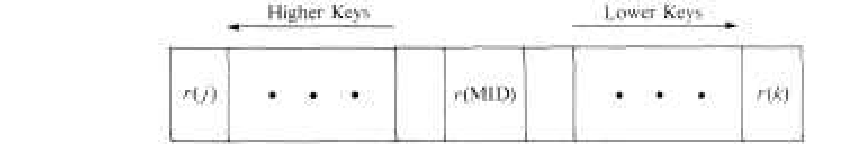
\includegraphics[width=1\linewidth]{images/fig-binsearch.png}
\caption{Example of a Binary Search
                \label{fig-binsearch}}
\end{figure}
\par
In the following algorithm, \(\textrm{Found}\) and \(\textrm{location}\) are ``global'' variables to execution of the algorithm.%
\begin{lstlisting}[style=genericinput, language=R]
def BinarySearch (j, k):
  Found = False
  if j < k: 
		Mid = floor( j + k ) / 2
		if r(Mid).key == C: 
	   	location = Mid
         Found = True
         Exit
	   else:
	   	if r(Mid).key < C:
				BinarySearch(j, Mid - 1)
			else: 
         	BinarySearch(Mid + 1 , k)
   else:
   	Exit
\end{lstlisting}
\typeout{************************************************}
\typeout{Subsection 1.1.4 Recursively Devined Sequences}
\typeout{************************************************}
\subsection[Recursively Devined Sequences]{Recursively Devined Sequences}\label{ss-recursive-sequences}
\index{Sequences!Recursively Defined}For the next two examples, consider a sequence of numbers to be a list of numbers consisting of a zeroth number, first number, second number, ... . If a sequence is given the name \(S\), the \(k^{th}\) number of \(S\), is usually written \(S_k\)  or \(S(k)\).%
\begin{example}[Geometric Growth Sequence]\label{ex-geometric-growth}
 Define the sequence of numbers \(B\) by
\begin{equation*}  B_0 = 100\textrm{ and }\end{equation*}  
\begin{equation*}  B_k = 1.08 B_{k-1} \textrm{ for } k\geq 1 \end{equation*}%
\par
These rules stipulate that each number in the list is 1.08 times the previous number, with the starting number equal to 100. For example

\begin{equation*}
\begin{split}
B_3 &= 1.08 B_2 \\
	&=1.08\left(1.08B_1\right)\\
	&= 1.08\left(1.08\left(1.08 B_0\right)\right)\\
	& = 1.08(1.08(1.08\cdot 100))\\
	&= 1.08^3 100 = 125.971
\end{split}
\end{equation*}
%
\end{example}
\begin{example}[The Fibonacci Sequence]\label{ex-fibonacci-sequence}
\index{Fibonacci Sequence}The Fibonacci sequence is the sequence \(F\) defined by 

\begin{equation*}F_0= 1 \textrm{, } F_1= 1\textrm{ and}\end{equation*} 

\begin{equation*}F_k = F_{k-2} + F_{k-1} \textrm{ for }k\geq 2\end{equation*}
%
\end{example}
\typeout{************************************************}
\typeout{Subsection 1.1.5 Recursion}
\typeout{************************************************}
\subsection[Recursion]{Recursion}\label{ss-recursion}
All of the previous examples were presented recursively. That is, every ``object'' is described in one of two forms. One form is by a simple
definition, which is usually called the basis for the recursion. The second form is by a recursive description in which objects are described in
terms of themselves, with the following qualification. What is essential for a proper use of recursion is that the objects can be
expressed in terms of simpler objects, where ``simpler'' means closer to the basis of the recursion. To avoid what might be considered a circular
definition, the basis must be reached after a finite number of applications of the recursion.%
\par
To determine, for example, the fourth item in the Fibonacci sequence we repeatedly apply the recursive rule for \(F\) until we are left
with an expression involving \(F_0\) and \(F_1\):

\begin{equation*}
\begin{split}
F_4 &= F_2+F_3\\	
	&=\left(F_0+F_1\right)+\left(F_1+F_2\right)\\
	&=\left(F_0+F_1\right)+\left(F_1+\left(F_0+F_1\right)\right)\\
	&=(1+1)+(1+(1+1))\\
	&=5
\end{split}
\end{equation*}
%
\typeout{************************************************}
\typeout{Subsection 1.1.6 Iteration}
\typeout{************************************************}
\subsection[Iteration]{Iteration}\label{ss-iteration}
On the other hand, we could compute a term in the Fibonacci sequence, say \(F_5\) by starting with the basis terms and working forward as follows:%
\leavevmode%
\begin{table}
\centering
\begin{tabular}{l}
\(F_2= F_0+ F_1 =1 + 1 =2\)\tabularnewline[0pt]
\(F_3= F_1+ F_2=1+ 2=3\)\tabularnewline[0pt]
\(F_4= F_2+F_3=2+3=5\)\tabularnewline[0pt]
\(F_5=F_3+F_4= 3+5=8\)
\end{tabular}
\end{table}
\par
This is called an iterative computation of the Fibonacci sequence. Here we start with the basis and work our way forward to a less simple number,
such as. Try to compute \(F_5\) using the recursive definition for F as we did for \(F_4\) . It will take much more time than it would have taken to do the computations above. Iterative computations usually tend to be faster than computations that apply recursion. Therefore, one useful skill is being able to convert a recursive formula into a nonrecursive formula, such as one that requires only iteration or a faster method, if possible.%
\par
An iterative formula for \(C(n, k)\) is also much more efficient than an application of the recursive definition. The recursive definition is not
without its merits, however. First, the recursive equation is often useful in manipulating algebraic expressions involving binomial
coefficients. Second, it gives us an insight into the combinatoric interpretation of \(C(n, k)\). In choosing \(k\) elements from \(\{1, 2,
. . . , n\}\), there are \(C(n - 1, k)\) ways of choosing all \(k\) from \(\{1,2, . . . ,n - 1\}\), and there are \(C(n -1;k-1)\) ways of choosing
the \(k\) elements if \(n\) is to be selected and the remaining \(k - 1\) elements come from \(\{1, 2, . . . , n - 1\}\). Note how we
used the Law of Addition from Chapter 2 in our reasoning.%
\par
\emph{BinarySearch Revisited.} In the binary search algorithm, the place where recursion is used is easy to pick out. When an item is examined and
the key is not the one you want, the search is cut down to a sublist of no more than half the number of items that you were searching in before.
Obviously, this is a simpler search. The basis is hidden in the algorithm. The two cases that complete the search can be thought of as the basis.
Either you find an item that you want, or the sublist that you have been left to search in is empty \(j > k\).%
\par
BinarySearch can be translated without much difficulty into any language that allows recursive calls to its subprograms. The advantage to such a program is that its coding would be much shorter than a nonrecursive program that does a binary search. However, in most cases the recursive version will be slower and require more memory at execution time.%
\typeout{************************************************}
\typeout{Subsection 1.1.7 Induction and Recursion}
\typeout{************************************************}
\subsection[Induction and Recursion]{Induction and Recursion}\label{ss-induction-and-recursion}
\index{Induction and Recursion}The definition of the positive integers in terms of Peano's Postulates is a recursive definition. The basis element is the number 1
and the recursion is that if n is a positive integer, then so is its successor. In this case, n is the simple object and the recursion is of a forward
type. Of course, the validity of an induction proof is based on our acceptance of this definition. Therefore, the appearance of induction proofs
when recursion is used is no coincidence.%
\begin{example}[Proof of a formula for \(B\)]\label{ex-geometric-squence-proof}
A formula for the sequence \(B\) in \hyperref[ex-geometric-growth]{Example~\ref{ex-geometric-growth}} is \(B = 100(1.08)^k\) for \(k\geq 0\). A proof by induction follow.%
\par
If \(k= 0\), then \(B = 100(1.08)^0 = 100\), as defined. Now assume that for some \(k\geq 1\), the formula for \(B_k\) is true.

\begin{equation*}
\begin{split}
B_{k+1} &= 1.08B_k \textrm{  by the recursive definition}\\
	&=1.08\left(100 (1.08)^k\right) \textrm{  by the induction hypothesis}\\ 
	&= 100 (1.08)^{k+1}
\end{split}
\end{equation*}
hence the formula is true for \(k+1\)%
\par
The formula that we have just proven for \(B\) is called a closed form expression. It involves no recursion or summation signs.%
\end{example}
\begin{definition}[Closed Form Expression.]\label{def-closed-form-expression}
\index{Closed Form Expression.} Let \(E = E\left(x_1, x_2, \ldots ,x_n\right)\) be an algebraic expression involving variables
\(x_1, x_2, \ldots ,x_n\) which are allowed to take on values from some predetermined set. \(E\) is a \textit{ closed form expression} if there exists
a number \(B\) such that the evaluation of \(E\) with any allowed values of the variables will take no more than \(B\) operations (alternatively, \(B\) time units).%
\end{definition}
\begin{example}[Reducing a summation to closed form]\label{ex-summation-simplifed}
The sum \(E(n)=\sum_{k=1}^n k\) is not a closed form expression because the number of additions needed evaluate \(E(n)\) grows indefinitely with \(n\). A closed form expression that computes the value of \(E(n)\) is \(\frac{n(n+1)}{2}\), which only requires \(B=3\) operations. %
\end{example}
\typeout{************************************************}
\typeout{Exercises 1.1.8 Exercises for Section 8.1}
\typeout{************************************************}
\subsection[Exercises for Section 8.1]{Exercises for Section 8.1}\label{exercises-1}
\hypertarget{exercisegroup-1}{}\typeout{************************************************}
\typeout{Introduction  }
\typeout{************************************************}
A Exercises%
\begin{exercisegroup}
\item[1.]\hypertarget{exercise-1}{}By the recursive definition of binomial coefficients, \(C(7, 2) = C(6, 2) + C(6, 1)\). Continue expanding \(C(7, 2)\) to express it in terms of quantities defined by the basis. Check your result by applying the factorial definition of \(C(n, k)\).%
\par\smallskip
\par\smallskip
\noindent\textbf{Answer.}\hypertarget{answer-1}{}\quad
\begin{equation*}
\begin{split}
 C(7,2)&=C(6,2)+C(6,1)\\
	&=C(5,2)+C(5,1)+C(5,1)+C(0,0)\\
&=C(5,2)+2 C(5,1)+1\\
&=C(4,2)+C(4,1)+2(C(4,1)+C(4,0))+1\\
&=C(4,2)+3 C4,1) + 3\\
&=C(3,2)+C(3,1)+3(C(3,1)+C(3,0))+3\\
&=C(3,2)+4 C(3,1) + 6\\
&=C(2,2)+C(2,1)+ 4(C(2,1)+C(2,0)) + 6\\
&=5 C(2,1)+ + 11\\
&=5(C(1,1)+C(1,0)) + 11\\
&=21
\end{split}
\end{equation*}
%
\item[2.]\hypertarget{exercise-2}{} Define the sequence \(L\) by \(L_0 = 5\) and for \(k\geq 1\), \(L _k = 2L_{k-1}-7\).  Determine \(L_4\) and prove
by induction that \(L_k=7-2^{k+1}\).%
\par\smallskip
\item[3.]\hypertarget{exercise-3}{} Let \(p(x) = x^5+ 3x^4 - 15x^3 + x - 10\).%
\par
\leavevmode%
\begin{enumerate}[label=\alph*]
\item\hypertarget{li-8}{} Write \(p(x)\) in telescoping form.%
\item\hypertarget{li-9}{} Use a calculator to compute \(p(3)\) using the original form of \(p(x)\). %
\item\hypertarget{li-10}{} Use a calculator to compute \(p(3)\) using the telescoping form of \(p(x)\).%
\item\hypertarget{li-11}{} Compare your speed in parts b and c.%
\end{enumerate}
%
\par\smallskip
\par\smallskip
\noindent\textbf{Answer.}\hypertarget{answer-2}{}\quad
\leavevmode%
\begin{enumerate}[label=\alph*]
\item\hypertarget{li-12}{} \(p(x)\) in telescoping form: \(((((x+3)x-15)x+0)x+1)x-10\)%
\item\hypertarget{li-13}{} \(p(3)=((((3+3)3-15)3-0)3+1)3-10=74\)%
\end{enumerate}
%
\end{exercisegroup}
\par\smallskip\noindent
\hypertarget{exercisegroup-2}{}\typeout{************************************************}
\typeout{Introduction  }
\typeout{************************************************}
B Exercises%
\begin{exercisegroup}
\item[4.]\hypertarget{exercise-4}{} Suppose that a list of nine items, (r(l), r(2), . . . , r(9)), is sorted by key in decending order so that \(r(3).\textrm{key} = 12\) and \(r(4).\textrm{key} = 10\). List the executions of the BinarySearch algorithms that would be needed to complete BinarySearch(1,9) for:%
\par
\leavevmode%
\begin{multicols}{2}
\begin{enumerate}[label=\alph*]
\item\hypertarget{li-14}{} C = 12%
\item\hypertarget{li-15}{} C = 11%
\end{enumerate}
\end{multicols}
%
\par
Assume that distinct items have distinct keys.%
\par\smallskip
\item[5.]\hypertarget{exercise-5}{} What is wrong with the following definition of \(f:\mathbb{R}\to \mathbb{R}\)? 
\(f(0) = 1\) and \(f(x) = f(x/2)/2\) if \(x\neq 0\).%
\par\smallskip
\par\smallskip
\noindent\textbf{Answer.}\hypertarget{answer-3}{}\quad
The basis is not reached in a finite number of steps if you try to compute \(f(x)\) for a nonzero value of \(x\).%
\item[6.]\hypertarget{exercise-6}{}Prove the two definitions of binomials coefficients, {$\langle\langle$Unresolved xref, reference "binomial-coefficient"; check spelling or use "provisional" attribute$\rangle\rangle$} and \hyperref[def-binomial-coefficient-recursive]{Definition~\ref{def-binomial-coefficient-recursive}}, are equivalent.%
\par\smallskip
\end{exercisegroup}
\par\smallskip\noindent
\typeout{************************************************}
\typeout{Section 1.2 Sequences}
\typeout{************************************************}
\section[Sequences]{Sequences}\label{s-Sequences}
\index{Sequences}\begin{definition}[Sequence]\label{def-sequence}
\index{Sequence}A sequence is a function from the natural numbers into some predetermined set. The image of any natural number \(k\) can be written  as \(S(k)\) or \(S_k\) and is called the \(k^{th}\)  \emph{term}  of \(S\). The variable
\(k\) is called the  \emph{index}  or  \emph{argument}  of the sequence.
%
\end{definition}
For example, a sequence of integers would be a function \(S:\mathbb{N}\to \mathbb{Z}\).%
\begin{example}[Three sequences defined in different ways]\label{ex-three-sequences}
\leavevmode%
\begin{enumerate}[label=\alph*]
\item\hypertarget{li-16}{} The sequence \(A\) defined by \(A(k) = k^2 - k\),  \(k \geq  0\), is a sequence of integers.%
\item\hypertarget{li-17}{} The sequence \(B\) defined recursively by \(B(0) = 2\) and \(B(k) = B(k - 1) + 3\) for\(k \geq  1\) is a sequence of integers. The terms of \(B\) can be computed either by applying the recursion formula or by iteration. For example;

\(\text{         }B(3) = B(2) + 3\quad =(B(1)+3)+3\quad = ((B(0)+3)+3)+3)\\
\\
\text{    }=((2+3)+3)+3\\
\\
\text{    }=11\)

or
\[B(1) = B(0) + 3 = 2 + 3 = 5\\
B(2) = B(1) + 3 = 5 + 8 = 8\\
B(3) = B(2) + 3 = 8 + 3 = 11\]%
\item\hypertarget{li-18}{}Let \(C_r\) be the number of strings of 0's and 1's of length \(r\) having no consecutive zeros. These terms define a sequence \(C\) of integers.%
\end{enumerate}
%
\end{example}
\par
Remarks:%
\par
\leavevmode%
\begin{enumerate}[label=\arabic*]
\item\hypertarget{li-19}{}A sequence is often called a  \emph{discrete function}.%
\item\hypertarget{li-20}{}Although it is important to keep in mind that a sequence is a function, another useful way of visualizing a sequence is as a list. For example,
the sequence \(A\) in the previous example could be written as \((0, 0, 2, 6, 12, 20, \dots )\). Finite sequences can appear much the same way when they are the input to or output from a computer. The index of a sequence can be thought of as a time variable. Imagine the terms of a sequence flashing on a screen every second. Then \(s_k\) would be what you see in the \(k^{th}\) second. It is convenient to use terminology like this in describing sequences.
For example, the terms that precede the \(k^{th}\) term of \(A\) would be \(A (0), A(1), . . . , A(k -1)\).  They might be called the earlier terms.%
\end{enumerate}
%
\par
\emph{A Fundamental Problem}%
\par
Given the definition of any sequence, a fundamental problem that we will concern ourselves with is to devise a method for determining any specific term in a minimum amount of time. Generally, time can be equated with the number of operations needed. In counting operations, the application of a recursive formula would be considered an operation.%
\par
\leavevmode%
\begin{enumerate}[label=\alph*]
\item\hypertarget{li-21}{} The terms of \(A\) in \hyperref[ex-three-sequences]{Example~\ref{ex-three-sequences}} are very easy to compute because of the closed form expression. No matter what term you decide to
compute, only three operations need to be performed.%
\item\hypertarget{li-22}{} How to compute the terms of \(B\) is not so clear. Suppose that you wanted to know \(B(100)\). One approach would be to apply the definition
recursively: \[B(100) = B(99) + 3 = (B(98) + 3) + 3 =\cdots\]
The recursion equation for \(B\) would be applied 100 times and 100 additions would then follow. To compute \(B(k)\) by this
method, \(2k\) operations are needed. An iterative computation of \(B(k)\) is an improvement: 

\(B(1) =B(0) +3 = 2 + 3 = 5\\
\\
B(2) =B(1)+3= 5 + 3 = 8\\
\\
\text{etc}.\)

Only \(k\) additions are needed. This still isn't a good situation. As \(k\) gets large, we take more and more time to compute \(B(k)\).  The formula \(B(k)=B(k-1)+3\) is called a recurrence relation on \(B\). The process of finding a closed form expression for
\(B(k)\), one that requires no more than some fixed number of operations, is called solving the recurrence relation.
%
\item\hypertarget{li-23}{} The determination of \(C_k\) is a standard kind of problem in combinatorics. One solution is by way of a recurrence relation. In fact, many problems in combinatorics are most easily solved by first searching for a recurrence relation and then solving it. The following
observation will suggest the recurrence relation that we need to determine \(C_k\). If \(k \geq  2\), then every string of 0's and 1's with length
\(k\) and no two consecutive 0's is either \(1s_{k-1}\) or \(01s_{k-2}\), where \(s_{k-1}\) and \(s_{k-2}\) are strings with no two consecutive
0's of length \(k - 1\) and \(k - 2\) respectively. From this observation we can see that \(C_k= C_{k-2}+C_{k-1}\) for \(k\geq 2\). The terms \(C_0=
1\) and \(C_1 = 2\) are easy to determine by enumeration. Now, by iteration, any \(C_k\) can be easily determined. For example, \(C_5 = 21\) can be computed with five additions. A closed form expression for \(C_k\) would be an improvement. Note that the recurrence relation for \(C_k\) is identical to the one for \hyperref[ex-fibonacci-sequence]{The Fibonacci Sequence}. Only the basis is different.%
\end{enumerate}
%
\typeout{************************************************}
\typeout{Exercises 1.2.1 Exercises for Section 8.2}
\typeout{************************************************}
\subsection[Exercises for Section 8.2]{Exercises for Section 8.2}\label{exercises-8-2}
\hypertarget{exercisegroup-3}{}\typeout{************************************************}
\typeout{Introduction  }
\typeout{************************************************}
A Exercises%
\begin{exercisegroup}
\item[1.]\hypertarget{exercise-7}{} Prove by induction that \(B(k) = 3k + 2,\) \(k\geq 0\), is a closed form expression for the sequence \(B\) in \hyperref[ex-three-sequences]{Example~\ref{ex-three-sequences}}%
\par\smallskip
\par\smallskip
\noindent\textbf{Answer.}\hypertarget{answer-4}{}\quad
Basis: \(B(0)=3\cdot 0+2=2\), as defined.%
\par
Induction: Assume: \(B(k)=3k+2\) for some \(k\geq 0\).

\begin{equation*}
\begin{split}
B(k+1) &=B(k)+3\\
		&=(3k+2)+3\quad \textrm{ by the induction hypothesis} \\
		&=(3k+3)+2\\
		&=3(k+1)+2\quad \textrm{as desired}
\end{split}
\end{equation*}
%
\item[2.]\hypertarget{exercise-8}{}\leavevmode%
\begin{enumerate}[label=\alph*]
\item\hypertarget{li-24}{}Consider sequence \(Q\) defined by \(Q(k) = 2k + 9\), \(k \geq  1\). Complete the table below and determine a recurrence relation
that describes \(Q\). 



\(\begin{array}{ccc}
 k & \text{     }Q(k)\text{     } & Q(k)-Q(k-1) \\
 2 &   &   \\
 3 &   &   \\
 4 & \text{  } &   \\
 5 &   &   \\
 6 &   &   \\
 7 &   &   \\
\end{array}\)
%
\item\hypertarget{li-25}{} Let \(A(k) = k^2 - k\), \(k \geq  0\). Complete the table below and determine a recurrence relation for \(A\) . Notice
that  \((A(k)-A(k-1)-(A(k-1)-A(k-2)) =A(k)-2A(k-1)+A(k-2)\)



 \(\begin{array}{cccc}
 k & \text{  }A(k)\text{       } & A(k)-A(k-1)\text{       } & A(k)-2A(k-1)+A(k-2) \\
 2 &   &   &   \\
 3 &   &   &   \\
 4 &   &   &   \\
 5 &   &   &   \\
\end{array}\)
%
\end{enumerate}
%
\par\smallskip
\item[3.]\hypertarget{exercise-9}{} Given \(k\) lines (\(k\geq 0\)) on a plane such that no two lines are parallel and no three lines meet at the same point, let \(P(k)\)
be the number of regions into which the lines divide the plane (including the infinite ones (see \hyperref[exercise-8-2-3]{Figure~\ref{exercise-8-2-3}}). Describe how the recurrence
relation \(P(k) = P(k - 1) + k\) can be derived. Given that \(P(0) = 1\), and determine \(P(5)\).
%
\leavevmode%
\begin{figure}
\centering
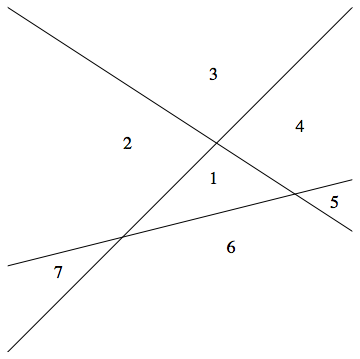
\includegraphics[width=1\linewidth]{images/exercise-8-2-3.png}
\caption{A general configuration of three lines\label{exercise-8-2-3}}
\end{figure}
\par\smallskip
\par\smallskip
\noindent\textbf{Answer.}\hypertarget{answer-5}{}\quad
Imagine drawing line \(k\) in one of the infinite regions that it passes through. That infinite region is divided into two infinite regions by line \(k\). As line \(k\) is drawn through every one of the \(k-1\) previous lines, you enter another region that line \(k\) divides. Therefore \(k\) regions are divided and the number of regions is increased by \(k\). %
\item[4.]\hypertarget{exercise-10}{} A sample of a radioactive substance is expected to decay by 0.15 percent each hour. If \(w_t,\) \(t \geq  0\), is the weight of the sample
\(t\) hours into an experiment, write a recurrence relation for \(w\).%
\par\smallskip
\end{exercisegroup}
\par\smallskip\noindent
\hypertarget{exercisegroup-4}{}\typeout{************************************************}
\typeout{Introduction  }
\typeout{************************************************}
B Exercise%
\begin{exercisegroup}
\item[5.]\hypertarget{exercise-11}{} Let \(M(n)\) be the number of multiplications needed to evaluate an \(n^{th}\) degree polynomial. Use the recursive definition of a
polynomial expression to define \(M\) recursively.%
\par\smallskip
\par\smallskip
\noindent\textbf{Answer.}\hypertarget{answer-6}{}\quad
For \(n\) greater than zero, \(M(n)=M(n-1)+1\), and \(M(0)=0\).%
\end{exercisegroup}
\par\smallskip\noindent
\typeout{************************************************}
\typeout{Section 1.3 Recurrence Relations}
\typeout{************************************************}
\section[Recurrence Relations]{Recurrence Relations}\label{s-recurrence-relations}
\typeout{************************************************}
\typeout{Introduction  }
\typeout{************************************************}
In this section we will begin our study of recurrence relations and their solutions. Our primary focus will be on the class of finite order linear
recurrence relations with constant coefficients (shortened to finite order linear relations). First, we will examine closed form
expressions from which these relations arise. Second, we will present an algorithm for solving them. In later sections we will consider some other
common relations (8.4) and introduce two additional tools for studying recurrence relations: generating functions (8.5) and matrix methods (Chapter
12).%
\typeout{************************************************}
\typeout{Subsection 1.3.1 Definition and Terminology}
\typeout{************************************************}
\subsection[Definition and Terminology]{Definition and Terminology}\label{defs-rr}
\begin{definition}[ Recurrence Relation.]\label{def-recurrence-relation}
\index{Recurrence Relation}Let S be a sequence of numbers, A recurrence relation on \(S\) is a formula that relates all but a finite number of terms of \(S\) to previous terms of \(S\). That is, there is a \(k_0\) in the domain of \(S\) such that if \(k \geq  k_0\), then \(S(k)\)
is expressed in terms of some (and possibly all) of the terms that precede \(S(k)\). If the domain of \(S\) is \(\{0,1,2,\textrm{...}\}\), the terms \(S
(0), S(1), . . . , S\left(k_0-1\right)\) are not defined by the recurrence formula.Their values are the initial conditions (or boundary conditions,
or basis) that complete the definition of \(S\).%
\end{definition}
\begin{example}[Some Examples of Recurrence Relations]\label{ex-some-recurrence-relations}
\leavevmode%
\begin{enumerate}[label=\alph*]
\item\hypertarget{li-26}{} The Fibonacci sequence is defined by the recurrence relation \(F_k= F_{k-2}+ F_{k-1}\),\(k\geq 2,\) with the initial conditions \(F_0=1\) and \(F_1=1\). The recurrence relation is called a second-order relation because \(F_k\) depends on the two previous terms of
\(F\). Recall that the sequence \(C\) in Section 8.2, \hyperref[ex-three-sequences]{\ref{ex-three-sequences}}, can be defined with the same recurrence relation, but with different initial conditions.%
\item\hypertarget{li-27}{} The relation \(T(k) = 2T(k - 1)^2 - k T(k - 3)\) is a third-order recurrence relation. If values of \(T(0)\), \(T(1)\), and \(T(2)\)
are specified, then \(T\) is completely defined.%
\item\hypertarget{li-28}{} The recurrence relation \(S(n) = S(\lfloor n/2\rfloor ) + 5\), \(n > 0\), with \(S(0)=0\) has infinite order. To determine \(S(n)\) when \(n\) is even, you must go back \(n/2\) terms. Since   \(n/2\)grows unbounded with \(n\), no finite order can be given to \(S\).%
\end{enumerate}
%
\end{example}
\typeout{************************************************}
\typeout{Subsection 1.3.2 Solving Recurrence Relations}
\typeout{************************************************}
\subsection[Solving Recurrence Relations]{Solving Recurrence Relations}\label{ss-solving-recurrence-relations}
\index{Recurrence Relations!Solving}Sequences are often most easily defined with a recurrence relation; however, the calculation of terms by directly applying a recurrence relation
can be time consuming. The process of determining a closed form expression for the terms of a sequence from its recurrence relation is called solving
the relation. There is no single technique or algorithm that can be used to solve all recurrence relations. In fact, some recurrence relations cannot
be solved. The relation that defines \(T\) above is one such example. Most of the recurrence relations that you are likely to encounter in
the future as classified as finite order linear recurrence relations with constant coefficients. This class is the one that we will spend most of
our time with in this chapter.%
\begin{definition}[\(n^{th}\) Order Linear Recurrence Relation]\label{def-n-th-order-rr}
\index{Order of a Recurrence Relation}Let S be a sequence of numbers with domain \(k\geq 0\).An \(n^{\textrm{th}}\)
order linear recurrence relation on S with constant coefficients is a recurrence relation that can be written in the form

\[S(k) + C_1 S(k - 1) + . . . + C_n S(k - n) = f(k)\textrm{  for  }k \geq  n\]

where \(C_1, C_2, \ldots , C_n\) are constants and \(f\) is a numeric function that is defined for \(k \geq n\).%
\end{definition}
\par
Note: We will shorten the name of this class of relations to \(n^{\textrm{th}}\) order linear relations. Therefore, in further discussions, \(S(k)
+ 2k S(k - 1) = 0\) would not be considered a first-order linear relation.%
\begin{example}[Some Finite Order Linear  Relations]\label{ex-some-finite-order-rr}
\leavevmode%
\begin{enumerate}[label=\alph*]
\item\hypertarget{li-29}{}The Fibonacci sequence is defined by the second-order linear relation because \(F_k- F_{k-1}- F_{k-2}=0\)%
\item\hypertarget{li-30}{} The relation \(P(j) + 2P(j - 3) = j^2\) is a third-order linear relation.In this case, \(C_1= C_2= 0\).%
\item\hypertarget{li-31}{} The relation \(A(k)= 2(A(k - 1) + k)\) can be written as \(A(k) - 2A(k - 1) = 2k\). Therefore, it is a first-order linear relation.
%
\end{enumerate}
%
\end{example}
\typeout{************************************************}
\typeout{Subsection 1.3.3 recurrence relations obtained from ``solutions''}
\typeout{************************************************}
\subsection[recurrence relations obtained from ``solutions'']{recurrence relations obtained from ``solutions''}\label{sss-recurrence-relations-obtained-from-solutions}
\index{Recurrence relations obtained from ``solutions''}Before giving an algorithm for solving finite order linear relations, we will examinerecurrence relations that arise from certain closed form
expressions. The closed form expressions are selected so that we will obtain finite order linear relations from them. This approach
may seem a bit contrived, but if you were to write down a few simple algebraic expressions, chances are that most of them would be similar to the
ones we are about to examine.%
\par
For our first example, consider D, defined by \(D(k) =5\cdot 2^k\), \(k \geq  0\). If \(k \geq  1\),

\(\quad\)\(D(k) =5\cdot 2^k = 2\cdot 5\cdot 2^{k-1} = 2 D(k - 1)\).

Therefore, \(D\) satisfies the first order linear relation \(D(k) - 2 D(k - 1) = 0\) and the initial condition \(D(0) = 5\) serves as an initial
condition for \(D\).%
\par
As a second example, consider \(C(k) =3^{k-1}+2^{k+1}+k\) , \(k \geq  0\). Quite a bit more algebraic manipulation is required to get our result:%
\leavevmode%
\begin{table}
\centering
\begin{tabular}{ll}\hrulethick
\(C(k) =3^{k-1}+2^{k+1}+k\)&Original equation\tabularnewline[0pt]
\(3C(k-1) =3^{k-1}+3\cdot 2^k+3(k-1)\)&\( \textrm{Substitute } k-1 \textrm{ for } k \textrm{ and multipy by } 3\)\tabularnewline[0pt]
\(\)&Subtract the second equation from the first\tabularnewline[0pt]
\(C(k)-3C(k-1)=-2^k-2k+3\)&\(3^{k-1} \textrm{ term  is eliminated. This is  a  first order relation.} \)\tabularnewline[0pt]
\(2C(k-1)-6C(k-2)=-2^k-2(2(k-1)+3)\)&\(\textrm{Substitute } k-1 \textrm{ for } k \textrm{ in the third equation, mult. by 2.}\)\tabularnewline[0pt]
\(\)&Subtract the fourth equation from the third equation.\tabularnewline[0pt]
\( C(k)-5C(k-1)-6C(k-2)=2k-7\)&\(2^{k+1}\textrm{term is eliminated. This is 2nd order relation.}\)
\end{tabular}
\end{table}
\par
The recurrence relation that we have just obtained, defined for \(k \geq  2\), together with the initial conditions \(C(0) = 7/3\) and \(C(1) = 5\),
define \(C\). We could do more algebra to derive a third-order linear relation in this case.
%
\par
\hyperref[table-reverse-solutions-rr]{Table~\ref{table-reverse-solutions-rr}} summarizes our results together with a few other examples that we will let the reader derive. Based on these results, we might conjecture
that any closed form expression for a sequence that combinesexponential expressions and polynomial expressions will be solutions of finite order
linear relations. Not only is this true, but the converse is true: a finite order linear relation defines a closed form expression that is similar
to the ones that were just examined. The only additional information that is needed is a set of initial conditions.%
\leavevmode%
\begin{table}
\centering
\begin{tabular}{cc}\hrulethick
Closed Form Expression&Recurrence Relation\tabularnewline[0pt]
\(D(k)=5\cdot 2^k\)&\(D(k)-2D(k-1)=0\)\tabularnewline[0pt]
\(C(k)=3^{k-1}+2^{k+1}+k\)&\(C(k)-2C(k-1)-6C(k-2)=2k-7\)\tabularnewline[0pt]
\(Q(k)=2k + 9\)&\(Q(k)-Q(k-1)=2\)\tabularnewline[0pt]
\(A(k)=k^2-k\)&\(A(k)-2A(k-1)+A(k-2)=2\)\tabularnewline[0pt]
\(B(k)=2 k^2+1\)&\(B(k)-2B(k-1)+B(k-2)=4\)\tabularnewline[0pt]
\(G(k)=2\cdot 4^k-5(-3)^k\)&\(G(k)-G(k-1)+12G(k-2)=0\)\tabularnewline[0pt]
\(J(k)=(3+k) 2^k\)&\(J(k)-4J(k-1)+4J(k-2)=0\)
\end{tabular}
\caption{Recurrence Relation Obtained from Certain Sequences\label{table-reverse-solutions-rr}}
\end{table}
\begin{definition}[ Homogeneous Recurrence Relation]\label{def-homogeneous-recurrence-relation}
\index{Homogeneous Recurrence Relation.}An \(n^{th}\) order linear relation is homogeneous if \(f(k)
= 0\) for all k.For each recurrence relation \(S(k) + C_1S(k - 1) +\ldots + C_n S(k - n) = f(k)\), the associated homogeneous relation is \(S(k)
+ C_1S(k - 1) +\ldots + C_n S(k - n) =0\)
%
\end{definition}
\begin{example}[First Order Homogeneous Recurrence Relations]\label{ex-first-order-homogeneous-rr}
\(D(k) - 2D(k - 1) = 0\) is a first-order homogeneous relation. Since it can also be written as \(D(k) =
2D(k - 1)\), it should be no surprise that it arose from an expression that involves powers of 2 (see Example 8.3.3a). More generally, you would
expect that the solution of \(L(k) - a L(k - 1)\) would involve \(a^k\) . Actually, the solution is \(L(k) = L(0)a^k\) , where the value of \(L(0)\)
is given by the the initial condition.
%
\end{example}
\begin{example}[A Second Order Example]\label{ex-second-order-rr}
 Consider the second-order homogeneous relation \(S(k) - 7S(k - 1) + 12 S(k- 2) = 0\) together with the initial conditions
\(S(0) = 4\) and \(S(1) = 4\). From our discussion above, we can predict that the solution to this relation involves terms of the form \(b a^k\),
where \(b\) and \(a\) are nonzero constants that must be determined. If the solution were to equal this quantity exactly, then

\[\quad \quad \quad  \begin{array}{ccc}
 S(k)=b a^k &   &   \\
 S(k-1)=b a^{k-1} & \textrm{   } & \textrm{  } \\
 S(k-2)=b a^{k-2} &   &   \\
\end{array}\]

Substitute these expressons into the recurrence relation to get


\[ b a^k-7 b a^{k-1}+12 b a^{k-1}=0\]

Each term on the left-hand side of this equation has a factor of \(b a^{k-2}\), which is nonzero. Dividing through by this common factor yields

\begin{gather}
-a^2 - 7a + 12 = -(a - 3) (a - 4) = 0\label{eq-characteristic-example}
\end{gather}%
\par
Therefore, the only possible values of \(a\) are 3 and 4. Equation \hyperref[eq-characteristic-example]{(\ref{eq-characteristic-example})} is called the characteristic equation of the recurrence relation.
The fact is that our original recurrence relation is true for any sequence of the form \(S(k) = b_1 3^k + b_24^k\), where \(b_1\) and \(b_2\) are
real numbers. This set of sequences is called the general solution of the recurrence relation. If we didn't have initial conditions for \(S\), we would stop here. The initial conditions make it possible for us to find definite values for \(b_1\) and \(b_2\).

 \[\left\{
\begin{array}{c}
 S(0)=4 \\
 S(1)=4 \\
\end{array}
\right\}\textrm{  }\Rightarrow \left\{
\begin{array}{c}
 b_13^0+b_24^0=4 \\
 b_13^1+b_24^1=4 \\
\end{array}
\right\}\textrm{  }\Rightarrow \left\{
\begin{array}{c}
 b_1+b_2=4 \\
 3b_1+4b_2=4 \\
\end{array}
\right\}\textrm{  }\]
%
\par
The solution of this set of simultaneous equations is \(b_1 = 12\) and \(b_2 = -8\) and so the solution is \(S(k) = 12 \cdot 3^k - 8 \cdot 4^k\).
%
\end{example}
\begin{definition}[Characteristic Equation]\label{def-characteristic-equation.}
\index{Characteristic Equation}\index{Characteristic Roots}The characteristic equation of the homogeneous \(n^{\textrm{th}}\) order linear relation \(S(k) + C_1 S(k- 1) +\ldots + C_n S(k - n) =0\)is the nth degree polynomial equation

\[a^n+\sum_{j=1}^n C_j a^{n-j}=a^n+ C_1a^{n-1}+\cdots +C_{n-1}x+C_n=0\] 

The left-hand side of this equation is called the characteristic polynomial.  The roots of the characteristic polynomial are called the characteristic roots of the equation%
\end{definition}
\begin{example}[Some characteristic equations]\label{ex-some-char-equations}
\leavevmode%
\begin{enumerate}[label=\alph*]
\item\hypertarget{li-32}{}The characteristic equation of \(F(k) - F(k - 1) - F(k - 2) = 0\) is \(a^2-a-1=0\).%
\item\hypertarget{li-33}{} The characteristic equation of \(Q(k) + 2Q(k - 1) - 3Q(k - 2) - 6 Q(k- 4) = 0\) is \(a^4+ 2a^3 - 3a^2 - 6 = 0.\)Note that the absence of
a \(Q(k - 3)\) term means that there is not an \(x^{4-3}=x\) term appearing in the characteristic equation.%
\end{enumerate}
%
\end{example}
\begin{algorithm}[Algorithm for Solving Homogeneous Finite-order Linear Relations]\label{algorithm-linear-homogeneous-recurrence-relations}

\leavevmode%
\begin{enumerate}
\item\hypertarget{li-34}{}Write out the characteristic equation of the relation \(S(k) + C_1S(k - 1) +\ldots + C_n S(k - n) =0\), which is \(a^n+ C_1a^{n-1}+\cdots
+C_{n-1}x+C_n=0\).%
\item\hypertarget{li-35}{}Find all roots of the characteristic equation, the characteristic roots.%
\item\hypertarget{li-36}{} If there are \(n\) distinct characteristic roots, \(a_1, a_2, \dots a_n\), then the general solution of the recurrence relation
is \(S(k) = b_1a_1{}^k+ b_2a_2{}^k+\cdots +b_na_n{}^k\). If there are fewer than \(n\) characteristic roots, then at least one root is a multiple
root. If \(a_j\) is a double root, then the \(b_ja_j{}^k\) term is replaced with \(\left(b_{j 0}+b_{j 1}k\right)a_j{}^k\). In general, if \(a_j\)
is a root of multiplicity \(p\), then the \(b_ja_j{}^k\) term is replaced with \(\left(b_{j 0}+b_{j 1}k+\cdots +b_{j(p-1)}k^{p-1}\right)a_j{}^k\).%
\item\hypertarget{li-37}{}If \(n\) initial conditions are given, we get \(n\) linear equations in \(n\) unknowns (the \(b_j's\) from Step 3) by substitution. If possible, solve these equations to determine a final form for \(S(k)\).%
\end{enumerate}

%
\end{algorithm}
\par
Although this algorithm is valid for all values of \(n\), there are limits to the size of \(n\) for which the algorithm is feasible. Using just a pencil and paper, we can always solve second-order equations. The quadratic formula for the roots of \(a x^2 + b x + c = 0\) is
\[x=\frac{-b\pm \sqrt{b^2-4 a c}}{2 a}\]
The solutions of \(a^2+ C_1a + C_2 = 0\) are then
\[\frac{1}{2}\left(-C_1+\sqrt{C_1{}^2-4 C_2}\right)\textrm{ and }\frac{1}{2}\left(-C_1-\sqrt{C_1{}^2-4 C_2}\right)\]
%
\par
Although cubic and quartic formulas exist, they are too lengthy to introduce here. For this reason, the only higher-order relations (\(n\geq 3\))
that you could be expected to solve by hand are ones for which there is an easy factorization of the characteristic polynomial.%
\begin{example}[A solution using the algorithm]\label{ex-hrr-solution-example-1}
 Suppose that \(T\) is defined by \(T(k) =7T(k-1)-10T(k-2)\), with , \(T(0) = 4\) and \(T(1) = 17\). We can solve this
recurrence relation with Algorithm 8.3.1:%
\par
\leavevmode%
\begin{enumerate}[label=\alph*]
\item\hypertarget{li-38}{}Note that we had written the recurrence relation in ``nonstandard'' form. To avoid errors in this easy step, you might consider a rearrangement
of the equation to, in this case, \(T(k) -7T(k-1)+10T(k-2)=0\).Therefore, the characteristic equation is \(a^2 -7a + 10 = 0\). %
\item\hypertarget{li-39}{} The characteristic roots are\(\frac{1}{2}\left(7+\sqrt{49-40}\right)=5\) and \(\frac{1}{2}\left(7-\sqrt{49-40}\right)=2\). These roots can be
just as easily obtained by factoring the characteristic polynomial into \((a - 5)(a - 2)\).%
\item\hypertarget{li-40}{}The general solution of the recurrence relation is \(T(k) =b_12^k+ b_25^k\) ,%
\item\hypertarget{li-41}{} \(\quad\) \(\left\{
\begin{array}{c}
 T(0)=4 \\
 T(1)=17 \\
\end{array}
\right\}\textrm{  }\Rightarrow \left\{
\begin{array}{c}
 b_12^0+b_25^0=4 \\
 b_12^1+b_25^1=4 \\
\end{array}
\right\}\textrm{  }\Rightarrow \left\{
\begin{array}{c}
 b_1+b_2=4 \\
 2b_1+5b_2=17 \\
\end{array}
\right\}\textrm{  }\)

The simultaneous equations have the solution \(b_1=1\) and \(b_2=3\), Therefore, \(T(k)=2^{k }+3\cdot 5^k\).%
\end{enumerate}
%
\end{example}
\par
Here is one rule that might come in handy: If the coefficients of the characteristic polynomial are all integers, with the constant
term equal to \(m\), then the only possible rational characteristic roots are divisors of \(m\) (both positive and negative).%
\par
With the aid of a computer (or possibly only a calculator), we can increase \(n\). Approximations of the characteristic roots can be obtained
by any of several well-known methods, some of which are part of standard software packages. There is no general rule that specifies the values of
\(n\) for which numerical approximations will be feasible. The accuracy that you get will depend on the relation that you try to solve. (See
Exercise 17 of this section.)%
\begin{example}[Solution of a Third Order Recurrence Relation.]\label{ex-hrr-solution-example-2}
 Solve \(S(k) - 7S(k - 2) + 6S(k - 3) = 0\), where \(S(0) =8\), \(S(1) = 6\), and \(S(2) = 22\).%
\par
\leavevmode%
\begin{enumerate}[label=\alph*]
\item\hypertarget{li-42}{} The characteristic equation is \(a^3 - 7a + 6 = 0\).%
\item\hypertarget{li-43}{}The only rational roots that we can attempt are \(\pm  1, \pm 2, \pm 3, \textrm{and} \pm 6\). By checking these, we obtain the three roots 1,
2, and $-$3.%
\item\hypertarget{li-44}{}The general solution is \(S(k) =b_11^k+b_22^k+b_3(-3){}^k\). The first term can simply be written \(b_1\) .

%
\item\hypertarget{li-45}{}\(\left\{
\begin{array}{c}
 S(0)=8 \\
 S(1)=6 \\
 S(20=22 \\
\end{array}
\right\}\textrm{   }\Rightarrow \left\{
\begin{array}{c}
 b_1+b_2+b_3=8 \\
 b_1+2b_2-3b_3=6 \\
 b_1+4b_2+9b_3=22 \\
\end{array}
\right\}\textrm{  }\)

You can solve this system by elimination to obtain \(b_1=5\), \(b_2=2\), and \(b_3=1\). Therefore,

\(\quad\)\(S(k) = 5 + 2\cdot 2^k + (-3)^k = 5 + 2^{k+1} + (-3)^k\)
%
\end{enumerate}
%
\end{example}
\begin{example}[Solution with a Double Characteristic Root]\label{ex-hrr-solution-example-3}
Solve \(D(k) - 8D(k - I) + 16D(k - 2) = 0\), where \(D(2) = 16\) and \(D(3) = 80\).%
\par
\leavevmode%
\begin{enumerate}[label=\alph*]
\item\hypertarget{li-46}{} Characteristic equation; \(a^2- 8a + 16 = 0\).%
\item\hypertarget{li-47}{}\(a^2- 8a + 16 = (a - 4)^2\). Therefore, there is a double characteristic root, 4.%
\item\hypertarget{li-48}{}General solution: \(D(k) = \left(b_{10}+b_{11}k\right)4^k\).%
\item\hypertarget{li-49}{}\(\left\{
\begin{array}{c}
 D(2)=16 \\
 D(3)=80 \\
\end{array}
\right\}\textrm{  }\Rightarrow \left\{
\begin{array}{c}
 \left(b_{10}+b_{11}2\right)4^2=16 \\
 \left(b_{10}+b_{11}3\right)4^3=80 \\
\end{array}
\right\}\textrm{  } \\ \Rightarrow \left\{
\begin{array}{c}
 16b_{10}+32b_{11}=16 \\
 64b_{10}+192b_{11}=80 \\
\end{array}
\right\} \Rightarrow  \left\{
\begin{array}{c}
 b_{10}=\frac{1}{2} \\
 b_{11}=\frac{1}{4} \\
\end{array}
\right\}\)
%
\par
Therefore \(D (k) = (1/2 + (1/4) k) 4^k= (2 + k)4^{k-1}\).
%
\end{enumerate}
%
\end{example}
\typeout{************************************************}
\typeout{Subsection 1.3.4 Solution of Monhomogeneous Finite Order Linear Relations}
\typeout{************************************************}
\subsection[Solution of Monhomogeneous Finite Order Linear Relations]{Solution of Monhomogeneous Finite Order Linear Relations}\label{ss-solution-of-nonhomogeneous-relations}
\index{Nonhomogeneous of Finite Order Linear Relations!Solution}Our algorithm for nonhomogeneous relations will not be as complete as for the homogeneous case. This is due to the fact that different right-hand
sides (f(k)'s) call for different rules in obtaining a particular solution.%
\begin{algorithm}[Algorithm for Solving Nonhomogeneous Finite-order Linear Relations]\label{algorithm-linear-nonhomogeneous-recurrence-relations}
To solve the recurrence relation \(S(k) + C_1S(k - 1) +\ldots + C_n S(k - n) = f(k)\)%
\par
\leavevmode%
\begin{enumerate}[label=\alph*]
\item\hypertarget{li-50}{}Write the associated homogeneous relation and find its general solution (Steps (a) through (c) of Algorithm 8.3.1). Call this the homogeneous
solution, \(S^{(h)}(k)\).%
\item\hypertarget{li-51}{}Start to obtain what is called a particular solution,\(S^{(p)}(k)\) of the recurrence relation by taking an educated guess at the form
of a particular solu tion. For a large class of right-hand sides, this is not really a guess, since the particular solution is often
the same type of function as \(f(k)\) (see Table 8.3.2).%
\item\hypertarget{li-52}{}Substitute your guess from Step 2 into the recurrence relation. If you made a good guess, you should be able to determine the unknown coefficients
of your guess. If you made a wrong guess, it should be apparent from the result of this substitution, so go back to Step 2.%
\item\hypertarget{li-53}{}The general solution of the recurrence relation is the sum of the homogeneous and particular solutions. If no conditions are
given, then you are finished. If \(n\) initial conditions are given, they will translate to \(n\) linear equations in \(n\) unknowns
and solve the system, if possible, to get a complete solution.%
\end{enumerate}
%
\end{algorithm}
\leavevmode%
\begin{table}
\centering
\begin{tabular}{cc}\hrulethick
Right Hand Side&Form of Particular Solution\tabularnewline[0pt]
Constant, \(q\)&Constant, \(d\)\tabularnewline[0pt]
Linear Function, \(q_0+q_1 k\)&Linear Function, \(d_0+d_1 k\)\tabularnewline[0pt]
\(m^{th}\) degree polynomial, \(q_0+q_1k+\cdots +q_m k^m\)&\(m^{th}\) degree polynomial, \(d_0+d_1k+\cdots +d_m k^m\)\tabularnewline[0pt]
exponential function, \(q a^k\)&exponential function, \(d a^k\)
\end{tabular}
\caption{Particular solutions for given right-hand sides\label{tab-particular-sols}}
\end{table}
\begin{example}[Solution of a Nonhomogeneous First Order Recurrence Relation]\label{ex-nhrr-solution-example-1}
 Solve \(S(k) + 5S(k - 1) = 9\),with \(S(0) = 6\).%
\par
\leavevmode%
\begin{enumerate}[label=\alph*]
\item\hypertarget{li-54}{}The associated homogeneous relation,\(S(k) + 5S(k - 1) = 0\) has the characteristic equation \(a + 5 = 0\); therefore, \(a = -5\). The
homogeneous solution is \(S^{(h)}(k) =b (-5)^k\).%
\item\hypertarget{li-55}{}Since the right-hand side is a constant, we guess that the particular solution will be a constant, \(d\).%
\item\hypertarget{li-56}{} If we substitute \(S^{(p)}(k) = d\) into the recurrence relation, we get \(d + 5d = 9\), or \(6d = 9\). Therefore, \(S^{(p)}(k)=1.5\)%
\item\hypertarget{li-57}{} The general solution of the recurrence relation is 

\(\quad\)\(S(k)= S^{(h)}(k)+S^{(p)}(k) =b (-5)^k+1.5\)

The initial condition will give us one equation to solve in order to determine \(b\).

\(\quad\)\(S(0) = 6 \Rightarrow \textrm{   }b(-5)^0+ 1.5 = 6\textrm{   }\Rightarrow \textrm{    }b\textrm{  }+ 1.5 = 6\)

Therefore, \(b = 4.5\) and \(S(k) = 4.5(-5)^k + 1.5\).%
\end{enumerate}
%
\end{example}
\begin{example}[Solution of a Nonhomogeneous Second Order Recurrence Relation]\label{ex-nhrr-solution-example-2}
 Consider \(T(k) - 7T(k - 1) + 10T(k - 2) = 6 + 8k\) with \(T(0) = 1\) and \(T(1) = 2\).%
\par
\leavevmode%
\begin{enumerate}[label=\alph*]
\item\hypertarget{li-58}{}From Example 8.3.7, we know that \(T^{(h)}(k)=b_12^k+ b_25^k\).Caution:Don't apply the initial conditions to \(T^{(h)}\) until you
add \(T^{(p)}\)!%
\item\hypertarget{li-59}{}Since the right-hand side is a linear polynomial, \(T^{(p)}\) is linear; that is, \(T^{(p)}(k)=d_0+d_1k\).%
\item\hypertarget{li-60}{}Substitutioninto the recurrence relation yields:

\(\left(d_0+d_1k\right)-7\left(d_0+d_1(k-1)\right)+10\left(d_0+d_1(k-2)\right)=6+8k\)

\(\quad\)\(\Rightarrow  \left(4d_0-13d_1\right)+ \left(4d_1\right)k = 6 + 8 k\)

Two polynomials are equal only if their coefficients are equal. Therefore,



\(\quad\) \(\left\{
\begin{array}{c}
 4d_0-13d_1=6 \\
 4d_1=8 \\
\end{array}
\right\}\Rightarrow \left\{
\begin{array}{c}
 d_0=8 \\
 d_1=2 \\
\end{array}
\right\}\)%
\item\hypertarget{li-61}{}Use the general solution \(T(k) =b_12^k+ b_25^k+8+2k\)and the initial conditions to get a final solution:

 \(\quad\) \(\left\{
\begin{array}{c}
 T(0)=1 \\
 T(1)=2 \\
\end{array}
\right\}\textrm{  }\Rightarrow \left\{
\begin{array}{c}
 b_1+ b_2+8=1 \\
 2b_1+5b_2+10=2 \\
\end{array}
\right\}\textrm{  }\\
\\
\quad \quad \Rightarrow \left\{
\begin{array}{c}
 b_1+b_2=-7 \\
 2b_1+5b_2=-8 \\
\end{array}
\right\}\\
\\
\quad \quad \Rightarrow \left\{
\begin{array}{c}
 b_1=-9 \\
 b_2=2 \\
\end{array}
\right\}\textrm{  }\)
%
\par
Therefore,  \(T(k) =-9\cdot 2^k+ 2\cdot 5^k+8+2k\)
%
\end{enumerate}
%
\end{example}
\begin{note}[A quick note on interest rates]\label{note-1}
When a quantity, such as a savings account balance, is increased by some fixed percent, it is most easily
computed with a multipier.In the case of an \(8\%\) increase, the multier is 1.08 because any original amount \(A\), has \(0.08A\) added
to it, so that the new balance is \(A+0.08A = (1+0.08)A = 1.08 A\).%
\par
Another example is that if the interest rate is \(3.5\%\), the multiplier would be 1.035. This presumes that the interest is applied a the end
of year for \(3.5\%\) annual interest, often called \terminology{simple interest}. If the interest is applied monthly, and we assume a simplifed case
where each month has the same length, the multiplier after every month would be \(\left(1+\frac{0.35}{12}\right) \approx  1.0292\).After a
year passes, this multiplier would be applied 12 times, which is the same as multiplying by\(1.0292^{12}\approx 1.3556\). That increase from
1.035 to 1.3556 is the effect of \terminology{compound interest}.%
\end{note}
\begin{example}[A Sort of Annuity]\label{ex-a-novel-annuity}
 Suppose you open a savings account that pays an annual interest rate of \(8\%\). In addition, suppose you decide to deposit one dollar when you open the account, and you intend to double your deposit each year.Let \(B(k)\) be your balance after \(k\) years. \textit{
B} can be described by the relation \(B(k) = 1.08 B(k - 1) + 2^k\), with \(S(0) = 1\). If, instead of doubling the deposit each year, you deposited
a constant amount, \(q\), the \(2^k\) term would be replaced with \(q\), A sequence of regular deposits such as this is called an annuity.%
\par
Returning to the original situation,%
\par
\leavevmode%
\begin{enumerate}[label=\alph*]
\item\hypertarget{li-62}{}\(B^{(h)}(k)=b_1(1.08){}^k\)%
\item\hypertarget{li-63}{}\(B^{(p)}(k)\) should be of the form \(d 2^k\).%
\item\hypertarget{li-64}{}\(d 2^k = 1.08d 2^{k-1}+2^k\\
\\
\quad \Rightarrow \textrm{  }(2d) 2^{k-1} = 1.08d 2^{k-1}+ 2\cdot 2^{k-1}\\
\\
\quad \Rightarrow  2d = 1.08 d + 2\\
\\
\quad \Rightarrow \textrm{  }.92d = 2 \\
\\
\quad \Rightarrow \textrm{   }d= 2.174 \textrm{  }(\textrm{to the nearest thousandth})\)

Therefore \(B^{(p)}(k)=2.174\cdot  2^k\)%
\item\hypertarget{li-65}{} \(B(0) = 1 \Rightarrow \textrm{   }b_1+2.174 = 1\\
\\
\textrm{\(\quad\)     }\Rightarrow \textrm{   }b_1= -1.174\)
%
\par
Therefore,  \(B(k) = -1.174\cdot  1.08^k+ 2.174\cdot  2^k\).
 %
\end{enumerate}
%
\end{example}
\begin{example}[Matching Roots]\label{ex-matching-roots}
 Find the general solution to \(S(k) - 3 S(k - 1) - 4 S(k - 2) = 4^k\).%
\par
\leavevmode%
\begin{enumerate}[label=\alph*]
\item\hypertarget{li-66}{}The characteristic roots of the associated homogeneous relation are -1 and 4. Therefore, \(S^{(h)}(k)=b_1(-1){}^k+ b_2 4^k\).%
\item\hypertarget{li-67}{}A function of the form \(d 4^k\) will not be a particular solution of the nonhomogeneous relation since it solves the associated homogeneous
relation. When the right-hand side involves an exponential function with a base that equals a characteristic root,you should multiply your guess
at a particular solution by \(k\). Our guess at \(S^{(p)}(k)\) would then be \(d k 4^k\) . See \hyperref[obs-matching-base]{\ref{obs-matching-base}} for a more complete description of this rule.%
\item\hypertarget{li-68}{}Substitute \(d k 4^k\) into the recurrence relation for \(S(k)\):
\(\quad\)\(d k 4^k-3d (k-1) 4^{k-1}-4d (k-2) 4^{k-2}=4^k\\
\\
16d k 4^{k-2}-12d (k-1) 4^{k-2}-4d (k-2) 4^{k-2}=4^k\)

Each term on the left-hand side has a factor of \(4^{k-2}\) 

 \(\quad\) \(\textrm{I6} d k - 12d(k - 1) - 4d(k - 2) = 4^220 d = 16\textrm{   }\Rightarrow \textrm{   }d=0.8\)

Therefore, \(S^{(p)}(k) = 0.8 k\textrm{  }4^4\)%
\item\hypertarget{li-69}{}The general solution to the recurrence relation is

\[S(k) =b_1(-1){}^k+ b_2 4^k +0.8 k 4^k\]
%
\end{enumerate}
%
\end{example}
\begin{observation}[When the base of right-hand side is equal to a characteristic root]\label{obs-matching-base}
 If the right-hand side of a nonhomogeneous relation involves an exponential with base \(a\), and \(a\) is also a characteristic root
of multiplicity \(p\), then multiply your guess at a particular solution as prescribed in Table 8,3.2 by \(k^p\) , where \(k\) is the
index of the sequence.%
\end{observation}
\begin{example}[Examples of matching bases]\label{ex-base-match}
\leavevmode%
\begin{enumerate}[label=\alph*]
\item\hypertarget{li-70}{} If  \(S(k) - 9S(k - 1) + 20 S(k - 2) = 2\cdot 5^k\), the characteristic roots are 4 and 5.  Since 5 matches the base of the right side, \(S^{(p)}(k)\) will take the form \(d k 5^k\).%
\item\hypertarget{li-71}{} If \(S(n)- 6S(n - 1) + 9 S(n - 2) = 3^{n+1}\) the only characteristic root is 3, but it is a double root (multiplicity 2).Therefore, the
form of the particular solution is \(d n^2 3^n\).%
\item\hypertarget{li-72}{} If \(Q(j)-Q(j-1)-12Q(j-2)=(-3)^j+ 6\cdot 4^j\), the characteristic roots are -3 and 4. The form of the particular solution will
be \(d_1j (-3)^j+ d_2j\cdot 4^j\).%
\item\hypertarget{li-73}{} If \(S(k) - 9S(k - 1) + 8S(k- 2) = 9k + 1 = (9k + 1)1^k\), the characteristic roots are 1 and 8.If the right-hand side is a polynomial,
as it is in this case, then the exponential factor \(1^k\) can be introduced. The particular solution will take the form \(k\left(d_0+ d_1k\right)\).
%
\end{enumerate}
%
\end{example}
\par
We conclude this section with a comment on the situation in which the characteristic equation gives rise to complex roots. If we restrict the coefficients
of our finite order linear relations to real numbers, or even to integers, we can still encounter characteristic equations whose roots are complex.
Here, we will simply take the time to point out that our algorithms are still valid with complex characteristic roots, but the customary method for
expressing the solutions of these relations is different. Since an understanding of these representations requires some background in complex numbers,
we will simply suggest that an interested reader can refer to a more advanced treatment of recurrence relations (see also difference equations).%
\typeout{************************************************}
\typeout{Exercises 1.3.5 Exercises for Section 8.3}
\typeout{************************************************}
\subsection[Exercises for Section 8.3]{Exercises for Section 8.3}\label{exercises-8-3}
\hypertarget{exercisegroup-5}{}\typeout{************************************************}
\typeout{Introduction  }
\typeout{************************************************}
A Exercises%
\par

Solve the following sets of recurrence relations and initial conditions:%
\begin{exercisegroup}
\item[1.]\hypertarget{exercise-12}{}
\(S(k) - 10S(k - 1) + 9S(k - 2) = 0\), \(S(0) = 3\),\(S(1) = 11\)%
\par\smallskip
\par\smallskip
\noindent\textbf{Answer.}\hypertarget{answer-7}{}\quad
 \(S(k)=2+9^k\)%
\item[2.]\hypertarget{exercise-13}{} \(S(k) - 9S(k - 1) + 18S(k - 2) = 0\)\(S(0) = 0\),\(S(1) = 3\)%
\par\smallskip
\item[3.]\hypertarget{exercise-14}{}\(S(k) - 0.25S(k - 1) = 0\) , \(S(0) = 6\)%
\par\smallskip
\par\smallskip
\noindent\textbf{Answer.}\hypertarget{answer-8}{}\quad
 \(S(k)=6(1/4)^k\)%
\item[4.]\hypertarget{exercise-15}{} \(S(k) - 20S(k - 1) + 100S(k - 2) = 0\),\(S(0) = 2\),\(S(1) = 50\)%
\par\smallskip
\item[5.]\hypertarget{exercise-16}{} \(S(k) - 2S(k - 1) + S(k - 2) = 2 \textrm{ }S(0) = 25,\textrm{  }S(1) = 16\)%
\par\smallskip
\par\smallskip
\noindent\textbf{Answer.}\hypertarget{answer-9}{}\quad
 \(S(k)=k^2-10k+25\)%
\item[6.]\hypertarget{exercise-17}{}\(S(k) - S(k - 1) - 6S(k - 2) = -30 \textrm{ }S(0) = 7, S(1) = 10\)%
\par\smallskip
\item[7.]\hypertarget{exercise-18}{}\(S(k) - 5S (k - 1) = 5^k,\textrm{  }S(0) = 3\)%
\par\smallskip
\par\smallskip
\noindent\textbf{Answer.}\hypertarget{answer-10}{}\quad
 \(S(k)=(3+k)5^k\)%
\item[8.]\hypertarget{exercise-19}{}\(S(k) - 5S(k - 1) + 6S(k - 2) = 2,\textrm{  }S(0) = -1,\textrm{  }S(1) = 0\)%
\par\smallskip
\item[9.]\hypertarget{exercise-20}{}\(S(k) - 4S(k - 1) + 4S(k - 2) = 3k + 2^k.\textrm{  }S(0) = 1, S(1) = 1\)%
\par\smallskip
\par\smallskip
\noindent\textbf{Answer.}\hypertarget{answer-11}{}\quad
 \(S(k)=(12+3k)+\left(k^2+7k-22\right)2^{k-1}\)%
\item[10.]\hypertarget{exercise-21}{} \(S(k) = r S(k - 1) + a ,\textrm{  }S(0) = 0,\textrm{   }r, a \geq  0, r \neq  1\)%
\par\smallskip
\item[11.]\hypertarget{exercise-22}{} \(S(k) - 4S(k - 1) - 11S(k- 2)+ 30S(k - 3) = 0\), 
 \(S(0) = 0\),\(S(1) = -35,\textrm{  }S(2) = -85\)%
\par\smallskip
\par\smallskip
\noindent\textbf{Answer.}\hypertarget{answer-12}{}\quad
 \(P(k)=4(-3)^k+2^k-5^{k+1}\)%
\item[12.]\hypertarget{exercise-23}{}Find a closed form expression for \(P(k)\) in Exercise 3 of Section 8.2.%
\par\smallskip
\item[13.]\hypertarget{exercise-24}{}\leavevmode%
\begin{enumerate}[label=\alph*]
\item\hypertarget{li-74}{}Find a closed form expression for the terms of the Fibonacci sequence (see Example 8.1.4).%
\item\hypertarget{li-75}{}The sequence \(C\) was defined by \(C_r\) = the number of strings of zeros and ones with length \(r\) having no consecutive
zeros (Example 8.2.1(c)). Its recurrence, relation is the same as that of the Fibonacci sequence. Determine a closed form expression for \(C_r\),
\(r \geq  1\).%
\end{enumerate}
%
\par\smallskip
\par\smallskip
\noindent\textbf{Answer.}\hypertarget{answer-13}{}\quad
\leavevmode%
\begin{enumerate}[label=\alph*]
\item\hypertarget{li-76}{}The characteristic equation is a \(a^2-a-1=0\), which has solutions \(\alpha =\left.\left(1+\sqrt{5}\right)\right/2\) and \(\beta =\left.\left(1-\sqrt{5}\right)\right/2\), It is useful to point out that \(\alpha +\beta =1\) and \(\alpha -\beta =\sqrt{5}\). The general solution is

\(F(k)=b_1\alpha ^k+b_2\beta ^k\).

Using the initial conditions, we obtain the system: \(b_1+b_2=1\) and \(b_1\alpha +b_2\beta =1\). The solution to this system is

 \(b_1=\alpha /(\alpha -\beta )=\left.\left(5+\sqrt{5}\right)\right/2\sqrt{5}\)
and  \(b_2=\beta /(\alpha -\beta )=\left.\left(5-\sqrt{5}\right)\right/2\sqrt{5}\) %
\par
Therefore the final solution is

\(F(n)=\left(1\left/\sqrt{5}\right.\right)\left[\left(\left.\left(1+\sqrt{5}\right)\right/2\right)^{n+1}-\left(\left.\left(1-\sqrt{5}\right)\right/2\right)^{n+1}\right]\)%
\item\hypertarget{li-77}{} \(C_r=F(r+1)\)%
\end{enumerate}
%
\item[14.]\hypertarget{exercise-25}{}If \(S(n)=\sum_{j=1}^n g(j)\),\(n\geq 1\), then \(S\) can be described with the recurrence relation \(S(n) = S(n-1) + g(n)\). For
each of the following sequences that are defined using a summation, find a closed form expression:%
\par
\leavevmode%
\begin{enumerate}[label=\alph*]
\item\hypertarget{li-78}{} \(S(n) =\sum_{j=1}^n j\),\(n\geq 1\)%
\item\hypertarget{li-79}{}\(Q(n) = \sum_{j=1}^n j^2\), \(n\geq 1\)%
\item\hypertarget{li-80}{}\(P(n) =\)\(\sum_{j=1}^n \left(\frac{1}{2}\right)^j\),\(n\geq 0\)%
\item\hypertarget{li-81}{} \(T(n)= \sum_{j=1}^n j^3\), \(n\geq 1\)%
\end{enumerate}
%
\par\smallskip
\end{exercisegroup}
\par\smallskip\noindent
\hypertarget{exercisegroup-6}{}\typeout{************************************************}
\typeout{Introduction  }
\typeout{************************************************}
B Exercises%
\begin{exercisegroup}
\item[15.]\hypertarget{exercise-26}{}Let \(D(n)\) be the number of ways that the set \(\{1, 2, . . . , n\}\), \(n \geq  1\), can be partitioned into two nonempty subsets.%
\par
\leavevmode%
\begin{enumerate}[label=\alph*]
\item\hypertarget{li-82}{}Find a recurrence relation for \(D\). (Hint: It will be a first-order linear relation.)%
\item\hypertarget{li-83}{}Solve the recurrence relation.%
\end{enumerate}
%
\par\smallskip
\par\smallskip
\noindent\textbf{Answer.}\hypertarget{answer-14}{}\quad
\leavevmode%
\begin{enumerate}[label=\alph*]
\item\hypertarget{li-84}{} \(D(n)=2D(n-1)+1 \textrm{for} n \geq 2 \textrm{and} D(1)=0.\)%
\item\hypertarget{li-85}{} \(D(n)=2^{n-1}-1\)%
\end{enumerate}
%
\item[16.]\hypertarget{exercise-27}{}If you were to deposit a certain amount of money at the end of each year for a number of years, this sequence of payment would be called an
annuity (see Example 8.3.12,).%
\par
\leavevmode%
\begin{enumerate}[label=\alph*]
\item\hypertarget{li-86}{}Find a closed form expression for the balance or value of an annuity that consists of payments of \(q\) dollars at a rate of interest
of \(i\). Note that for a normal annuity, the first payment is made after one year.%
\item\hypertarget{li-87}{}With an interest rate of 12.5$\%$, how much would you need to deposit into an annuity to have a value of one million dollars after 18 years?%
\item\hypertarget{li-88}{}The payment of a loan is a form of annuity in which the initial value is some negative amount (the amount of the loan) and the annuity ends
when the value is raised to zero. How much could you borrow if you can afford to pay $\$$5,000 per year for 25 years at 14$\%$ interest?%
\end{enumerate}
%
\par\smallskip
\end{exercisegroup}
\par\smallskip\noindent
\hypertarget{exercisegroup-7}{}\typeout{************************************************}
\typeout{Introduction  }
\typeout{************************************************}
C Exercises%
\begin{exercisegroup}
\item[17.]\hypertarget{exercise-28}{}Suppose that \(C\) is a small positive number. Consider the recurrence relation \(B(k) - 2B(k - 1) + \left(1 - C ^2\right)B(k - 2)
= C^2\), with initial conditions \(B(0) = 1\) and \(B(1) = 1\). If \(C\) is small enough, we might consider approximating the relation by replacing
\(1 - C^2\) with 1 and \(C^2\) with 0. Solve the original relation and its approximation. Let \(B_a\) a be the solution of the approximation. Compare
closed form expressions for \(B(k)\) and \(B_a(k)\). Their forms are very different because the characteristic roots of the original relation were
close together and the approximation resulted in one double characteristic root.If characteristic roots of a relation
are relatively far apart, this problem will not occur. For example, compare the general solutions of 
\(\quad\)\(S(k) + 1.001S(k - 1) - 2.004002S(k - 2) = 0.0001\) and
\(\quad\)\(S_a(k) + S_a(k - 1) - 2S_a(k - 2) = 0\).%
\par\smallskip
\end{exercisegroup}
\par\smallskip\noindent
\typeout{************************************************}
\typeout{Section 1.4 Some Common Recurrence Relations}
\typeout{************************************************}
\section[Some Common Recurrence Relations]{Some Common Recurrence Relations}\label{s-some-common-rrs}
\typeout{************************************************}
\typeout{Introduction  }
\typeout{************************************************}
In this section we intend to examine a variety of recurrence relations that are not finite-order linear with constant coefficients. For each part of this section, we will consider a concrete example, present a solution, and, if possible, examine a more general form of the original relation.%
\typeout{************************************************}
\typeout{Subsection 1.4.1 A  First Basic Example}
\typeout{************************************************}
\subsection[A  First Basic Example]{A  First Basic Example}\label{rr-basic-example}
 Consider the homogeneous first-order linear relation without constant coefficients,  \(S(n) - n S(n - 1) = 0\), \(n \geq  1\), with initial condition \(S(0)
= 1\). Upon close examination of this relation, we see that the \(n\)th term is \(n\) times the \((n - 1)^{st}\) term, which is a property of \(n\) factorial.\(S(n) = n!\) is a solution of this relation, for if \(n \geq  1\),

\[S(n) = n! = n \cdot (n -1)! = n\cdot  S(n - 1)\]

In addition, since \(0! = 1\), the initial condition is satisfied. It should be pointed out that from a computational point of view, our ``solution''
really isn't much of an improvement since the exact calculation of \(n!\) takes \(n-1\) multiplications.%
\par
If we examine a similar relation, \(G(k) - 2 ^k G(k - 1),\) \(k\geq 1\) with \(G(0) = 1\), a table of values for \(G\) suggests a possible solution:

 \[\begin{array}{ccccccc}
 k & 0 & 1 & 2 & 3 & 4 & 5 \\
\hline
 G(k) & 1 & 2 & 2^3 & 2^6 & 2^{10} & 2^{15} \\
\end{array}\]

The exponent of 2 in \(G(k)\) is growing according to the relation \(E(k) = E(k - 1) + k,\) with \(E(0) = 0\). Thus \(E(k)=\frac{k(k+1)}{2}\)
and \(G(k) = 2^{k(k+1)/2}\) . Note that \(G(k)\) could also be written as \(2^0 2^1 2^2 \cdots 2^k\), for \(k \geq  0\), but this is not a closed form expression.%
\par
In general, the relation \(P(n) = f(n)P(n - 1)\) for \(n \geq 1\) with \(P(0) =f(0)\), where \(f\) is a function that is defined for all \(n\geq
0\), has the ``solution''


\[P(n)=\prod _{k=0}^n f(k)\]


This product form of \(P(n)\) is not a closed form expression because as \(n\) grows, the number of multiplications grow. Thus, it is really not a true solution.  Often, as for \(G(k)\) above, a closed form expression can be derived from the product form.%
\typeout{************************************************}
\typeout{Subsection 1.4.2 A Analysis of the Binary Search Algorithm.}
\typeout{************************************************}
\subsection[A Analysis of the Binary Search Algorithm.]{A Analysis of the Binary Search Algorithm.}\label{analysis-of-binary-search}
\typeout{************************************************}
\typeout{Subsubsection 1.4.2.1  }
\typeout{************************************************}
\subsubsection[ ]{ }\label{subsubsection-1}
 Suppose you intend to use a binary search algorithm (see \hyperref[ss-recursive-searching]{\ref{ss-recursive-searching}}) on lists of zero or more sorted items, and that the items are stored in an array, so that you have easy access to each item. A natural question to ask is ``How much time will it take to complete the search?'' When a question like this is asked, the time we refer to is often the so - called worst - case time. That is, if we were to search through \(n\) items, what is the longest amount of time that we will need to complete the search? In order to make an analysis such as this independent of the computer to be used, time is measured by counting the number of steps that are executed. Each
step (or sequence of steps) is assigned an absolute time, or weight; therefore, our answer will not be in seconds, but in absolute time units. If
the steps in two different algorithms are assigned weights that are consistent, then analyses of the algorithms can be used to compare their relative
efficiencies. There are two major steps that must be executed in a call of the binary search algorithm:%
\par
\leavevmode%
\begin{enumerate}[label=\arabic*]
\item\hypertarget{li-89}{} If the lower index is less than or equal to the upper index, then the middle of the list is located and its key is compared to the value that
you are searching for.%
\item\hypertarget{li-90}{}In the worst case, the algorithm must be executed with a list that is roughly half as large as in the previous execution. If we assume that
Step 1 takes one time unit and \(T(n)\) is the worst - case time for a list of \(n\) items, then

\begin{gather}
T(n)= 1 + T (\lfloor n/2 \rfloor ),  \quad n>0\label{eq-bin-search-recursion}
\end{gather}

For simplicity, we will assume that

\begin{gather}
T(0) = 0\label{eq-bin-search-basis}
\end{gather}


even though the conditions of Step 1 must be evaluated as false if \(n = 0\). You might wonder why \(n/2\) is truncated in \hyperref[eq-bin-search-recursion]{(\ref{eq-bin-search-recursion})}. If \(n\) is
odd, then \(n = 2 k + 1\) for some \(k\geq  0\), the middle of the list will be the \((k + 1)^{st}\)  item, and no matter what half of the list the search is directed to, the reduced list will have \(k = \lfloor n/2\rfloor\) items. On the other hand, if \(n\) is even, then \(n
= 2 k\) { }for \(k>0\). The middle of the list will be the \(k^{th}\) item, and the worst case will occur if we are directed to the \(k\) items
that come after the middle (the \((k + l)^{st}\) through \((2k)^{th}\) items). Again the reduced list has \(\lfloor n/2\rfloor\) items.%
\end{enumerate}
%
\par
\emph{Solution to \hyperref[eq-bin-search-recursion]{(\ref{eq-bin-search-recursion})}  and \hyperref[eq-bin-search-basis]{(\ref{eq-bin-search-basis})}.}  To determine \(T(n)\), the easiest case is when \(n\) is a power of two. If we compute \(T \left(2^m\right)\),
\(m\geq 0\) , by iteration, our results are

\begin{equation*}T(1) = \text{ }1 + T(0) = 1\\
\\
T(2) = \text{ }1 + T(1) = 2\\
\\
T(4) = \text{ }1 + T(2) = 3\\
\\
T(8) = \text{ }1 + T(4) = 4
\end{equation*}

The pattern that is established makes it clear that \(T\left(2^m\right) = m + 1\). This result would seem to indicate that every time you double the size of your list, the search time increases by only one unit.%
\par
A more complete solution can be obtained if we represent n in binary form. For each \(n\geq 1\), there exists a non-negative integer \(r\) such that

\begin{gather}
\quad \quad 2^{r-1}\leq n < 2^r\label{eq-inequality-84}
\end{gather} 

For example, if \(n = 21\), \(2^4 \leq  21 < 2^5\); therefore, \(r = 5\). If \(n\) satisfies (8.4c), its binary representation requires \textit{
r} digits. For example, \(21_{\text{ten}}\) = \(10101_{\textrm{two}}\).%
\par
In general, \(n = \left(a_1a_2\ldots  a_r\right)_{\textrm{two}}\). where \(a_1=1\). Note that in this form, \(\lfloor n/2\rfloor\) is easy to describe:
it is the \(r-1\) digit binary number \(\left(a_1a_2\ldots  a_{r-1}\right)_{\textrm{two}}\)%
\par
Therefore,

\begin{equation*}
\begin{split}
T(n) &= T\left(a_1a_2\ldots  a_r\right)\\
	& =1+ T\left(a_1a_2\ldots  a_{r-1}\right)\quad \\
	& =1+\left(1+ T\left(a_1a_2\ldots  a_{r-2}\right)\right)\\
	& =2+ T\left(a_1a_2\ldots  a_{r-2}\right)\\
	&\quad  \vdots \\
	& = (r-1) + T\left(a_1\right)\\
	& = (r-1)+1\quad \textrm{ since } T(1)=1\\
	& = r
\end{split}
\end{equation*}%
\par
From the pattern that we've just established, \(T(n)\) reduces to \(r\). A formal inductive proof of this statement is possible. However, we
expect that most readers would be satisfied with the argument above. Any skeptics are invited to provide the inductive proof. %
\par
For those who prefer to see a numeric example, suppose \(n = 21\).

\(\quad \quad \)\(T(21) = T(10101) \\
\\
\quad = 1 + T(1010) \\
\\
\quad = 1 + (1 + T(101)) \\
\\
\quad = 1 + (1 + (1 + T(10))) \\
\\
\quad = 1 + (1 + (1 + (1 + T(1))))\\
\\
\quad = 1 + (1 + (1 + (1 + (1 +T(0)))))\\
\\
\quad = 5\)
%
\par
Our general conclusion is that the solution to \hyperref[eq-bin-search-recursion]{(\ref{eq-bin-search-recursion})}  and \hyperref[eq-bin-search-basis]{(\ref{eq-bin-search-basis})} is that for \(n\geq 1\), \(T(n) = r\), where \(2^{r-1}\leq n < 2^r\).%
\par
A less cumbersome statement of this fact is that \(T(n)=\left\lfloor \log_{2}n\right\rfloor +1\). For example, { }\(T(21) = \left\lfloor \log_2 21\right\rfloor + 1 = 4 + 1 = 5\). %
\typeout{************************************************}
\typeout{Subsubsection 1.4.2.2 review of logarithms}
\typeout{************************************************}
\subsubsection[review of logarithms]{review of logarithms}\label{sss-review-of-logarithms}
\index{Review of logarithms}Any discussion of logarithms must start by establishing a base, which can be any positive number other than 1. With the exception of Theorem 8.4.1,
our base will be 2. We will see that the use of a different base (10 and \(e\approx  2.171828\) are the other common ones) only has the effect of
multiplying each logarithm by a constant. Therefore, the base that you use really isn't very important. Our choice of base 2 logarithms is convenient
for the problems that we are considering.%
\begin{definition}[Base 2 logarithm]\label{def-log-base-2}
\index{Logarithm, base 2}The base 2 logarithm of a positive number represents an exponent and is defined by the following equivalence for any positive real numbers \(a\).
\[\log_2 a = x \quad \Leftrightarrow \quad 2^x= a\]. %
\end{definition}
\leavevmode%
\begin{figure}
\centering
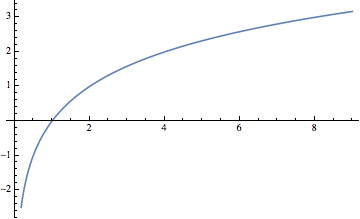
\includegraphics[width=1\linewidth]{images/fig-log-2-plot.png}
\caption{Plot of the logarithm, bases 2, function\label{fig-log-2-plot}}
\end{figure}
\par
For example, \(\log_2 8 = 3\) because \(2^3 = 8\) and \(\log_21.414\approx 0.5\) because \(2^{0.5}\approx 1.414\) . A graph of the function \(f(x)
= \log_2 x\) in \hyperref[fig-log-2-plot]{Figure~\ref{fig-log-2-plot}} shows that if \(a < b\), the \(\log_2a < \log_2 b\); that is, when \(x\) increases, \(\log_2 x\) also increases.
However, if we move \(x\) from \(2^{10} = 1024\) to \(2^{11} = 2048\), \(\log_2 x\) only increases from 10 to 11. This slow rate of increase
of the logarithm function is an important point to remember. An algorithm acting on \(n\) pieces of data that can be executed in \(\log_2{n}\)
time units can handle significantly larger sets of data than an algorithm that can be executed in \(n/100\) or  \(\sqrt{n}\) time units. The graph of \(T(n)=\left\lfloor \log_2n\right\rfloor +1\) would show the same behavior.%
\par
A few more properties that we will use in subsequent discussions involving logarithms are summarized in the following theorem.%
\begin{theorem}[Fundamental Properties of Logarithms]\label{theorem-log-properties}
\index{Logarithms!Properties}Let \(a\) and \(b\) be positive real numbers, and \(r\) a real number.

\begin{gather}
log_2 1 = 0\label{eq-log-prop-1}\\
log_2 a b = \log_2a + \log_2b\label{eq-log-prop-2}\\
log_2 \frac{a}{b}= \log_2a - \log_2b\label{eq-log-prop-3}\\
log_2a^r = r \log_2a\label{eq-log-prop-4}\\
2^{\log_2a}= a\label{eq-log-prop-5}
\end{gather}
%
\end{theorem}
\begin{definition}[ Logarithms base \(b\)]\label{def-logarithm-general-base}
\index{Logarithm!General Base}\label{notation-1}
If \(b > 0\), \(b \neq 1\), then for \(a>0\), 
 \[\log_b a = x\Leftrightarrow b^x= a\]%
\end{definition}
\begin{theorem}[How logarithms with different bases are related]\label{theorem-logs-related}
Let \(b>0\), \(b \neq 1\). Then for all \(a >0\), \(\log_b a = \frac{\log_2a}{\log_2b}\). Therefore, if \(b > 1\), base b logarithms can be computed from base 2 logarithms by dividing by the positive scaling factor \(\log_2b\). { }If \(b < 1\), this scaling factor is negative.%
\end{theorem}
\begin{proof}\hypertarget{proof-1}{}
By an analogue of \hyperref[eq-log-prop-5]{(\ref{eq-log-prop-5})}, \(a=b^{\log_b a}\). Therefore, if we take the base 2 logarithm of both sides of this equality we get:
\begin{equation*}\log_2 a = \log_2 \left(b^{\log_b a}\right)  \Rightarrow \log_2 a =\log_b a \cdot \log_2 b\end{equation*}
Finally, divide both sides of the last equation by \(\log_2b\). \(\square\)%
\end{proof}
\begin{note}[]\label{note-2}
 \(\log_210 \approx  3.32192\) and \(\log_2e = 1.55269\).%
\end{note}
\typeout{************************************************}
\typeout{Subsubsection 1.4.2.3  }
\typeout{************************************************}
\subsubsection[ ]{ }\label{subsubsection-3}
Returning to the binary search algorithm, we can derive the final expression for \(T(n)\) using the properties of logarithms, including that the
logarithm function is increasing so that inequalities are maintained when taking logarithms of numbers.%
\par

\begin{equation*}
\begin{split}
T(n)= r & \Leftrightarrow 2^{r-1}\leq n < 2^r\\
	& \Leftrightarrow  \log_2 2^{r-1} \leq \log_2 n < \log_2 2^r\\
	& \Leftrightarrow  r-1 \leq \log_2 n < r\\
	& \Leftrightarrow  r-1 = \lfloor \log_2 n\rfloor \\
	& \Leftrightarrow  T(n) = r= \left\lfloor \log_2 n\right\rfloor +1
\end{split}
\end{equation*}
%
\par
We can apply several of these properties of logarithms to get an alternate expression for \(T(n)\):
\begin{equation*}
\begin{split}
\left\lfloor \log_2n\right\rfloor +1 &= \left\lfloor \log_2n+1\right\rfloor \\
		& = \left\lfloor \log_2n + \log_22\right\rfloor \\
		&  =\text{  }\left\lfloor \log_22n \right\rfloor 
\end{split}
\end{equation*}
%
\par
If the time that was assigned to Step 1 of the binary search algorithm is changed, we wouldn't expect the form of the solution to be very different. If \(T(n)= a + T (\lfloor n/2 \rfloor )\) with \(T(0) = c\), then \(T(n) = c + a \left\lfloor \log_2{2n}\right\rfloor\).%
\par
A further generalization would be to add a coefficient to \(T(\lfloor n/2 \rfloor )\): \(T(n)= a + b T (\lfloor n/2 \rfloor )\) with \(T(0) = c\),
where \(a, b, c\in \mathbb{R}\), and \(b\neq 0\) is not quite as simple to derive. First, if we consider values of \(n\) that are powers of 2:



\begin{equation*}
T(1) = a + b T(0) = a + b c\\
\\
T(2)=a + b(a+b c) = a + a b +c b^2\\
\\
T(4)=a+b\left(a + a b +c b^2\right) = a + a b + a b^2+ c b^3\\
\\
\quad \vdots \\
\\
T\left(2^r\right) = a + a b + a b^2+\cdots  + a b^r + c b^{r+1}\end{equation*}



If \(n\) is not a power of 2, by reasoning that is identical to what we used to \hyperref[eq-bin-search-recursion]{(\ref{eq-bin-search-recursion})}  and \hyperref[eq-bin-search-basis]{(\ref{eq-bin-search-basis})},



 \[T(n) =\sum_{k=0}^r a b^k+ c b^{r+1}\]



where \(r = \left\lfloor \log_2n\right\rfloor\).%
\par
 The first term of this expression is a geometric sum, which can be written in closed form. Let \(x\) be that sum:

 \[x =\textrm{  }a + a b + a b^2+\cdots  + a b^r \\
   b x=\textrm{            }a b + a b^2+\cdots  + a b^r + a b^{r+1}\]

We've multiplied each term of \(x\) by \(b\) and aligned the identical terms in \(x\) and \( bx\). Now if we subtract the two equations,
\begin{equation*}x - b x = a - a b ^{r+1} \Rightarrow x(1-b) = a\left(1-b^{r+1}\right)\end{equation*} 
Therefore, \(x = a\frac{b^{r+1}-1}{b-1}\).%
\par
A closed form expression for \(T(n)\) is



\begin{equation*}T(n) = a\frac{b^{r+1}-1}{b-1} +\text{  }c b^{r+1}\text{  }\text{where}\text{  }r = \left\lfloor \log_2n\right\rfloor \text{  }\end{equation*}
%
\typeout{************************************************}
\typeout{Subsection 1.4.3 Analysis of Bubble Sort and Merge Sort}
\typeout{************************************************}
\subsection[Analysis of Bubble Sort and Merge Sort]{Analysis of Bubble Sort and Merge Sort}\label{ss-bubblesort-analysis}
\index{Bubble Sort}\index{Merge Sort}
 The efficiency of any search algorithm such as the binary search relies on fact that the search list is sorted according to a key value and that the search is based on the key value. There are several methods for sorting a list. One example is the bubble sort. You might
be familiar with this one since it is a popular ``first sorting algorithm.'' A time analysis of the algorithm shows that if \(B(n)\) is the worst-case
time needed to complete the bubble sort on \(n\) items, then \(B(n) =(n-1) + B(n-1)\) and \(B(1) = 0\). The solution of this relation is a
quadratic function \(B(n) =\frac{1}{2}\left(n^2-n\right)\). The growth rate of a quadratic function such as this one is controlled by its squared
term. Any other terms are dwarfed by it as \(n\) gets large. For the bubble sort, this means that if we double the size of the list that we
are to sort, \(n\) changes to \(2n\) and so \(n^2\) becomes \(4n^2\) . Therefore, the time needed to do a bubble sort is quadrupled. One alternative
to bubble sort is the merge sort. Here is a simple version of this algorithm for sorting \(F=\{r(1), r(2), \ldots , r(n)\}\), \(n \geq  1\). If \(n
= 1\), the list is sorted trivially. If \(n\geq  2\) then:%
\par
\leavevmode%
\begin{enumerate}[label=\arabic*]
\item\hypertarget{li-91}{} Divide \(F\) into \(F_1= \{r(1), \ldots , r(\lfloor n/2\rfloor )\}\) and \(F_2= \{r(\lfloor n/2\rfloor +1), \ldots ,r(n)\}\).%
\item\hypertarget{li-92}{}Sort \(F_1\) and \(F_2\) using a merge sort.%
\item\hypertarget{li-93}{}Merge the sorted lists \(F_1\) and \(F_2\) into one sorted list. If the sort is to be done in descending order of key values, you continue to choose the higher key value from the fronts of \(F_1\) and \(F_2\) and place them in the back of \(F\).%
\end{enumerate}
%
\par
Note that \(F_1\) will always have \(\lfloor n/2\rfloor\) items and \(F_2\) will have \(\lceil n/2\rceil\) items; thus, if \(n\) is odd, \(F_2\)
gets one more item than \(F_1\). We will assume that the time required to perform Step 1 of the algorithm is insignificant compared to the other
steps; therefore, we will assign a time value of zero to this step. Step 3 requires roughly \(n\) comparisons and \(n\) movements of
items from \(F_1\) and \(F_2\) to \(F\); thus, its time is proportional to \(n\). For this reason, we will assume that Step 3 takes
\(n\) time units. Since Step 2 requires \(T(\lfloor n/2\rfloor ) + T(\lceil n/2\rceil )\) time units,
\begin{gather}
T(n) = n + T(\lfloor n/2\rfloor ) + T(\lceil n/2\rceil )\label{mrow-10}
\end{gather}
with the initial condition
\begin{gather}
(T(1) = 0\label{mrow-11}
\end{gather}
%
\par
Instead of an exact solution of these equations, we will be content with an estimate for \(T(n)\).  First, consider the case of \(n=2^r\), \(r \geq 1\):



\begin{equation*}
T\left(2^1\right)= T(2) = 2 +T(1)+T(1)= 2 = 1\cdot  2\\
\\
T\left(2^2\right) = T(4)=4+\text{  }T(2)+T(2)=8 = 2\cdot 4\\
\\
T\left(2^3\right) =T(8)=8 + T(4)+T(4) =24=3\cdot 8\\
\\
\quad \vdots \\
\\
T\left(2^r\right)=r 2^r= 2^r \log_22^r
\end{equation*}
%
\par
Thus, if \(n\) is a power of 2, \(T(n) = n \log_2 n\). Now if, for some\(r \geq  2\), \(2^{r-1}\leq n\leq 2^r\) , then \((r-1)2^{r-1}\leq
T(n) < r 2^r\). This can be proven by induction on \(r\). As \(n\) increases from \(2^{r-1}\) to \(2^r\), \(T(n)\) increases from \((r-1)2^{r-1}\)to
\(r 2^r\) and is slightly larger than \(\left\lfloor n \log_2n\right\rfloor\). The discrepancy is small enough so that \(T_e(n)=\left\lfloor n \log
_2n\right\rfloor\) can be considered a solution of 8.4i and 8.4j for the purposes of comparing the merge sort with other algorithms. Table 8.4.1
compares \(B(n)\) with \(T_e(n)\) for selected values of \(n\).%
\leavevmode%
\begin{table}
\centering
\begin{tabular}{ccc}\hrulethick
n&\(B(n)\)&\(T_e(n)\)\tabularnewline[0pt]
10&45&34\tabularnewline[0pt]
50&1225&283\tabularnewline[0pt]
100&4950&665\tabularnewline[0pt]
500&124750&4483\tabularnewline[0pt]
1000&499500&9966
\end{tabular}
\caption{Comparison of Times for Bubble Sort and Merge Sort\label{table-sort-analysis}}
\end{table}
\typeout{************************************************}
\typeout{Subsection 1.4.4 Derangements}
\typeout{************************************************}
\subsection[Derangements]{Derangements}\label{ss-derangements}
\index{Derangement}A derangement is a permutation on a set that has no ``fixed points''.  Here is a formal definition:%
\begin{definition}[ Derangement.]\label{def-derangement.}
A derangement of a set A is a permutation of A (i.e., a bijection from A into A) such that \(f(a)\neq a\) for all \(a \in  A\).%
\end{definition}
\par
 If \(A = \{1, 2, . . . , n\}\), an interesting question might be ``How many derangements are there of \(A\)?''  We know that our answer is bounded above by \(n!\). We can also expect our answer to be quite a bit smaller than \(n!\) since \(n\) is the image of itself for \((n-1)!\) of the permutations of \(A\).%
\par
Let \(D(n)\) be the number of derangements of \(\{1, 2, . . . , n\}\). Our answer will come from discovering a recurrence relation on \(D\). Suppose that \(n \geq  3\). If we are to construct a derangement of \(\{1, 2, \dots , n\}\), \(f\), then \(f(n) = k \neq n\). Thus, the
image of \(n\) can be selected in \(n-1\) different ways. No matter which of the \(n -1\) choices we make, we can complete the definition of
\(f\) in one of two ways. First, we can decide to make \(f(k) = n\), leaving \(D(n -2)\) ways of completing the definition of \textit{
f}, since \(f\) will be a derangement of \(\{1, 2, \dots ,n\} - \{n, k\}\). Second, if we decide to select \(f(k)\neq  n\), each of the
\(D(n - 1)\) derangements of \(\{1, 2,\dots ,n-1\}\) can be used to define \(f\). If \(g\) is a derangement of \(\{1, 2, \dots , n-1\}\) such that \(g(p) = k\), then define f by

\[f(j)=\left\{
\begin{array}{cc}
 n & \textrm{ if } j = p \\
 k & \textrm{ if } j = n \\
 g(j) & \textrm{ otherwise } \\
\end{array}
\right.\]

%
\par
Note that with our second construction of \(f\), \(f(f(n)) = f(k) \neq  n\), while in the first construction, { }\(f(f(n)) = f(k) = n\). Therefore,
no derangement of \(\{1, 2, . . . , n\}\) with \(f(n) = k\) can be constructed by both methods.%
\par
To recap our result, we see that \(f\) is determined by first choosing one of \(n - 1\) images of \(n\) and then constructing the
remainder of \(f\) in one of \(D(n - 2) + D(n -1)\) ways. Therefore,

\begin{gather}
D(n) = (n - 1) (D(n - 2) + D(n - 1))\label{mrow-12}
\end{gather}
%
\par
This homogeneous second-order linear relation with variable coefficients, together with the initial conditions \(D(1) = 0\) and \(D(2) = 1\), completely
defines \(D\). Instead of deriving a solution of this relation by analytical methods, we will give an empirical derivation of an approximation of \(D(n)\). Since the derangements of \(\{1,2 . . . , n\}\) are drawn from a pool of \(n!\) permutations, we will see what percentage of these permutations
are derangements by listing the values of \(n!\), \(D(n)\), { }and \(\frac{D(n)}{n!}\).  The results we observe will indicate that
as \(n\) grows, \(\frac{D(n)}{n!}\) hardly changes at all. If this quotient is computed to eight decimal places, for \(n \geq  12\), \(D(n)/n!
= 0.36787944\). The reciprocal of this number, which \(D(n)/n!\) seems to be tending toward, is, to eight places, 2.71828182. This number appears
in so many places in mathematics that it has its own name, \(e\). An approximate solution of our recurrence relation on \(D\) is then \(D(n)\approx \frac{n!}{e}\)%
\par

\begin{equation*}\begin{array}{lll}
 \text{n} & \text{D(n)} & \text{D(n)/n!} \\
 1 & 0 & 0 \\
 2 & 1 & 0.50000000 \\
 3 & 2 & 0.33333333 \\
 4 & 9 & 0.37500000 \\
 5 & 44 & 0.36666667 \\
 6 & 265 & 0.36805556 \\
 7 & 1854 & 0.36785714 \\
 8 & 14833 & 0.36788194 \\
 9 & 133496 & 0.36787919 \\
 10 & 1334961 & 0.36787946 \\
 11 & 14684570 & 0.36787944 \\
 12 & 176214841 & 0.36787944 \\
 13 & 2290792932 & 0.36787944 \\
 14 & 32071101049 & 0.36787944 \\
 15 & 481066515734 & 0.36787944 \\
\end{array}
\end{equation*}
%
\typeout{************************************************}
\typeout{Exercises 1.4.5 Exercises for Section 8.4}
\typeout{************************************************}
\subsection[Exercises for Section 8.4]{Exercises for Section 8.4}\label{exercises-8-4}
\hypertarget{exercisegroup-8}{}\typeout{************************************************}
\typeout{Introduction  }
\typeout{************************************************}
A Exercises%
\begin{exercisegroup}
\item[1.]\hypertarget{exercise-29}{}Solve the following recurrence relations. Indicate whether your solution is an improvement over iteration.%
\par
\leavevmode%
\begin{enumerate}[label=\alph*]
\item\hypertarget{li-94}{} \(n S(n) - S(n - 1) = 0\), { }\(S(0) = 1\).%
\item\hypertarget{li-95}{} { }\(T(k) + 3k T(k - 1) = 0\), \(T(0) = 1\).%
\item\hypertarget{li-96}{} \(U(k) -\frac{k-1}{k}U(k - 1) = 0\), \(k \geq  2\), \(U(1) = 1\).%
\end{enumerate}
%
\par\smallskip
\par\smallskip
\noindent\textbf{Answer.}\hypertarget{answer-15}{}\quad
\leavevmode%
\begin{enumerate}[label=\alph*]
\item\hypertarget{li-97}{}  \(S(n)=1/n\)!  %
\item\hypertarget{li-98}{}\(U(k)=1/k\), an improvement. %
\item\hypertarget{li-99}{}  \(T(k)=(-3)^kk\)!, no improvement.%
\end{enumerate}
%
\item[2.]\hypertarget{exercise-30}{}Prove that if \(n \geq 0\), { }\(\lfloor n/2\rfloor +\lceil n/2\rceil = n\). (Hint: Consider the cases of n odd and n even separately.)
%
\par\smallskip
\end{exercisegroup}
\par\smallskip\noindent
\hypertarget{exercisegroup-9}{}\typeout{************************************************}
\typeout{Introduction  }
\typeout{************************************************}
B Exercises%
\begin{exercisegroup}
\item[3.]\hypertarget{exercise-31}{}Solve as completely as possible:%
\par
\leavevmode%
\begin{enumerate}[label=\alph*]
\item\hypertarget{li-100}{}\(T(n) = 3 + T(\lfloor n/2\rfloor )\), \(T(0) = 0\).%
\item\hypertarget{li-101}{}\(T(n) = 1 + \frac{1}{2}T(\lfloor n/2\rfloor )\), { }\(T(0) = 2\).%
\item\hypertarget{li-102}{} \(V(n) = 1 + V\lfloor n/8\rfloor )\), \(V(0) = 0\). (Hint: Write \(n\) in octal form.)%
\end{enumerate}
%
\par\smallskip
\par\smallskip
\noindent\textbf{Answer.}\hypertarget{answer-16}{}\quad
\leavevmode%
\begin{enumerate}[label=\alph*]
\item\hypertarget{li-103}{}  \(T(n)=3\left(\left\lfloor \log _2n\right\rfloor +1\right)\) %
\item\hypertarget{li-104}{} \(V(n)=\left\lfloor \log _8n\right\rfloor +1\)%
\item\hypertarget{li-105}{}\(T(n)=2\)%
\end{enumerate}
%
\item[4.]\hypertarget{exercise-32}{} Prove by induction that if \(T(n)= 1 + T (\lfloor n/2 \rfloor )\), \(T(0) = 0\), and \(2^{r-1}\leq n < 2^r\) , \(r \geq  1\), then \(T(n) = r\).
%
\par\smallskip
\par\smallskip
\noindent\textbf{Hint.}\hypertarget{hint-1}{}\quad
Prove by induction on \(r\).%
\item[5.]\hypertarget{exercise-33}{} Use the substitution \(S(n) = T(n + 1)/T(n)\) to solve
\(T(n)T(n-2)-T(n)^2=1\) for \(n \geq  2\), with \(T(0) = 1\), \(T(1) = 6\), and\(T(n) \geq  0\).%
\par\smallskip
\par\smallskip
\noindent\textbf{Answer.}\hypertarget{answer-17}{}\quad
 The indicated substitution yields \(S(n)=S(n+1)\). Since \(S(0)=T(1)/T(0)=6\), \(S(n)=6\) for all \(n\). Therefore \(T(n+1)=6T(n)\Rightarrow T(n)=6^n\).%
\item[6.]\hypertarget{exercise-34}{} Use the substitution \(G(n) =T(n)^2\) { }to solve
\(T(n)^2-T(n-1)^2=1\) for \(n \geq  1\), with \(T(0) = 10\).%
\par\smallskip
\item[7.]\hypertarget{exercise-35}{}Solve as completely as possible:%
\par
\leavevmode%
\begin{enumerate}[label=\alph*]
\item\hypertarget{li-106}{} \(Q(n)=1+Q\left(\left\lfloor \sqrt{n}\right\rfloor \right)\), \(n \geq  2\), \(Q(1) = 0\).%
\item\hypertarget{li-107}{} \(R(n)=n +R(\lfloor n/2\rfloor )\), \(n \geq  1\), \(R(0) = 0\).%
\end{enumerate}
%
\par\smallskip
\par\smallskip
\noindent\textbf{Answer.}\hypertarget{answer-18}{}\quad
\leavevmode%
\begin{enumerate}[label=\alph*]
\item\hypertarget{li-108}{} A good approximation to the solution of this recurrence relation
 is based on the following observation: \(n\) is a power of a power of two; that is,
  \(n\) is \(2^m\), where \(m=2^k\) , then \(Q(n)=1+Q\left(2^{m/2}\right)\).
   By applying this recurrence relation \(k\) times we obtain \(Q(n)=k\).
    Going back to the original form of \(n\),
     \(\log _2n=2^k\) or \(\log _2\left(\log _2n\right)=k\).
      We would expect that in general, \(Q(n)\) is \(\left\lfloor \log _2\left(\log _2n\right)\right\rfloor\).
       We do not see any elementary method for arriving at an exact solution. %
\item\hypertarget{li-109}{} Suppose that \(n\) is a positive integer with \(2^{k-1} \leq n < 2^k\).
 Then \(n\) can be written in binary form, \(\left(a_{k-1}a_{k-2}\cdots  a_2a_1a_0\right)_{\textrm{two}}\)
  with \(a_{k-1}=1\) and \(R(n)\) is equal to the sum \(\underset{i=0}{\overset{k-1}{\Sigma }}\)
  \(\left(a_{k-1}a_{k-2}\cdots  a_i\right)_{\textrm{two}}\). If \(2^{k-1}\leq n < 2^k\),
   then we can estimate this sum to be between \(2n-1\) and \(2n+1\).
    Therefore, \(R(n)\approx 2n\).%
\end{enumerate}
%
\item[8.]\hypertarget{exercise-36}{}Suppose Step 1 of the merge sort algorithm did take a significant amount of time. Assume it takes 0.1 time unit, independent of the value of
\(n\)%
\par
\leavevmode%
\begin{enumerate}[label=\alph*]
\item\hypertarget{li-110}{}Write out a new recurrence relation for \(T(n)\) that takes this factor into account.%
\item\hypertarget{li-111}{} Solve for \(T\left(2^r\right)\), \(r \geq  0\).%
\item\hypertarget{li-112}{}Assuming the solution for powers of 2 is a good estimate for all n, compare your result to the solution in the text. As gets large, is there
really much difference?%
\end{enumerate}
%
\par\smallskip
\end{exercisegroup}
\par\smallskip\noindent
\typeout{************************************************}
\typeout{Section 1.5 Generating Functions}
\typeout{************************************************}
\section[Generating Functions]{Generating Functions}\label{s-generating-functions}
\index{Generating Functions}\typeout{************************************************}
\typeout{Introduction  }
\typeout{************************************************}
This section contains an introduction to the topic of generating functions and how they are used to solve recurrence relations, among other problems.
Methods that employ generating functions are based on the concept that you can take a problem involving sequences and translate it into a problem
involving generating functions. Once you've solved the new problem, a translation back to sequences gives you a solution of the original problem.%
\par
This section covers:%
\par
\leavevmode%
\begin{enumerate}[label=\arabic*]
\item\hypertarget{li-113}{}The definition of a generating function;%
\item\hypertarget{li-114}{}Solution of a recurrence relation using generating functions to identify the skills needed to use generating functions;\\%
\item\hypertarget{li-115}{}An introduction and/or review of the skills identified in point b;\\%
\item\hypertarget{li-116}{}Some applications of generating functions.%
\end{enumerate}
%
\typeout{************************************************}
\typeout{Subsection 1.5.1 Definition}
\typeout{************************************************}
\subsection[Definition]{Definition}\label{ss-what-is-a-generating-function}
\begin{definition}[Generating Function of a Sequence]\label{def-generating-function}
\index{Generating Function}\label{notation-2}
The generating function of a sequence S with terms \(S_0,S_1 ,S_2, \dots \),  is the infinite sum
 \[G(S;z)=\sum_{n=0}^{\infty} S_n z^n=S_0+S_1 z+S_2 z^2+S_3 z^3+\cdots\]
The domain and codomain of generating functions will not be of any concern to us since we will only be performing algebraic operations on them.%
\end{definition}
\begin{example}[First Examples]\label{ex-first-gf-examples}
\leavevmode%
\begin{enumerate}[label=\alph*]
\item\hypertarget{li-117}{} If \(S_n = 3^n\),\(n \geq  0\), then

\(G(S;z) = 1 + 3z + 9z^2 + 27z^3 +\cdots \\
\\
\quad =\sum_{n=0}^{\infty} 3^n z^n\\
\\
\quad =\sum_{n=0}^{\infty} (3 z)^n\)

We can get a closed form expression for \(G(S;z)\) by observing that \(G(S;z) - 3z G(S;z) = 1\). Therefore,

\(G(S;z) =\frac{1}{1-3 z}\).%
\item\hypertarget{li-118}{}Finite sequences have generating functions. For example, the sequence of binomial coefficients \(C(n; 0)\), \(C(n; 1)\), \(\ldots\),\(C(n;
n)\), \(n \geq  1\) has generating function

\(G(C(n; \cdot ); z) = C(n; 0) + C(n; 1)z +\cdots  + C(n; n)z^n\\
\\
\quad \quad = \sum_{k=0}^{\infty} C(n;k) z^k\\
\\
\quad \quad =(1+z)^n\)

by application of the binomial formula.%
\item\hypertarget{li-119}{} If \(Q(n) = n^2\),

\(G(Q;z)=\sum_{n=0}^{\infty} n^2 z^n=\sum_{k=0}^{\infty} k^2 z^k\)

Note that the index that is used in the summation has no significance. Also, note that the lower limit of the summation could start at 1 since \(Q(0)=0\).%
\end{enumerate}
%
\end{example}
\typeout{************************************************}
\typeout{Subsection 1.5.2 Solution of a Recurrence Relation Using Generating Functions}
\typeout{************************************************}
\subsection[Solution of a Recurrence Relation Using Generating Functions]{Solution of a Recurrence Relation Using Generating Functions}\label{ss-solution-of-rr-using-generating-functions}
We illustrate the use of generating functions by solving
 \(S(n) - 2S(n - 1) - 3S(n - 2) = 0\), \(n \geq  2\), with \(S(0) = 3\) and \(S(1) = 1\).%
\par
\leavevmode%
\begin{enumerate}[label=\arabic*]
\item\hypertarget{li-120}{} Translate the recurrence relation into an equation about generating functions.%
\par
Let \(V(n) = S(n) - 2S (n - 1) - 3S (n - 2)\), \(n \geq  2\), with \(V(0) = 0\) and \(V(1) = 0\). Therefore,
\[G(V;z) = 0 + 0z +\sum_{n=2}^{\infty}  (S(n) - 2S (n - 1) - 3S (n - 2)) z^n= 0\]
%
\item\hypertarget{li-121}{}Solve for the generating function of the unknown sequence, \(G(S,z) = \sum_{n=0}^{\infty} S_n z^n\).
 \begin{equation*}
 \begin{split}
 0 & =\sum_{n=2}^{\infty}  {(S(n) - 2S (n - 1) - 3 S (n - 2)) z^n}\\
 	& =\sum_{n=2}^{\infty} {S(n) z^n-2} \left(\sum_{n=2}^{\infty
} S(n-1) z^n\right)-3\left(\sum_{n=2}^{\infty} S(n-2) z^n\right)
\end{split}
\end{equation*}
%
\par
Close examination of the three sums above shows:%
\par
%
\begin{enumerate}[label=\alph*]
\item\hypertarget{li-122}{}
\begin{equation*}
\begin{split}
\sum_{n=2}^{\infty} S_n z^n &=\sum_{n=0}^{\infty} S_n z^n - S(0)-S(1)z\\
			&= G(S;z)-3-z
\end{split}
\end{equation*}
since \(S(0)=3\) and \(S(1)=1\).%
\item\hypertarget{li-123}{}
\begin{equation*}
\begin{split}
\sum_{n=2}^{\infty} S(n-1) z^n &=z\left(\sum_{n=2}^{\infty} S(n-1) z^{n-1}\right)\\
		& =z\left(\sum_{n=1}^{\infty} S(n) z^n\right)\\
		& = z\left(\sum_{n=0}^{\infty} S(n) z^n-S(0)\right)\\
		&= z(G(S;z)-3
\end{split}
\end{equation*}
%
\item\hypertarget{li-124}{}
\begin{equation*}
\begin{split}
\sum_{n=2}^{\infty} S(n-2) z^n  & = z^2\left(\sum_{n=2}^{\infty} S(n-2) z^{n-2}\right)\\
	& =z^2G(S;z)
\end{split}
\end{equation*}
%
\par
Therefore, 
\begin{equation*}
\begin{split}
&(G(S;z)-3-z)-2z(G(S;z)-3)-3z^2G(S;z)=0\\
	 & \Rightarrow G(S;z)-2z G(S;z)-3z^2G(S;z)=3 - 5z\\
		&\Rightarrow G(S;z)=\frac{3-5z}{1-2z-3z^2}
\end{split}
\end{equation*}
%
\end{enumerate}
%
\item\hypertarget{li-125}{}Determine the sequence whose generating function is the one we got in Step 2.%
\par
For our example, we need to know one general fact about the closed form expression of an exponential sequence (a proof will be given later):
\begin{gather}
T(n)=b a^n ,n\geq 0 \Leftrightarrow G(T;z)=\frac{b}{1-a z} \label{gf-of-exp}
\end{gather}
%
\par
Now, in order to recognize \(S\) in our example, we must write our closed form expression for \(G(S;z)\) as a sum of terms like \(G(T;z)\) above. Note that the denominator of \(G(S;z)\) can be factored:

 \[G(S;z)=\frac{3-5z}{1-2z-3z^2} =\frac{3-5z}{(1-3z)(1+z)}\]

If you look at this last expression for \(G(S;z)\) closely, you can imagine how it could be the result of addition of two fractions,
\begin{gather}
\frac{3-5z}{(1-3z)(1+z)} = \frac{A}{1-3z}+ \frac{B}{1+z}
\label{eq-pf}
\end{gather}
where \(A\) and \(B\) are two real numbers that must be determined. Starting on the right of \hyperref[eq-pf]{(\ref{eq-pf})}, it should be clear that the sum, for
any \(A\) and \(B\), would look like the left-hand side. The process of finding values of \(A\) and \(B\) that make \hyperref[eq-pf]{(\ref{eq-pf})}
true is called the \terminology{partial fractions decomposition} of the left-hand side:

\begin{equation*}
\begin{split}
\frac{A}{1-3z}+ \frac{B}{1+z} &=\frac{A(1+z)}{(1-3z)(1+z)}+ \frac{B(1-3z)}{(1-3z)(1+z)}\\
		& =\frac{(A+B)+(A-3B)z}{(1-3z)(1+z)}
\end{split}
\end{equation*}
%
\par
Therefore,



 \[\left\{
\begin{array}{c}
 A+B=3 \\
 A-3B=-5 \\
\end{array}
\right\}\Rightarrow \left\{
\begin{array}{c}
 A=1 \\
 B=2 \\
\end{array}
\right\}\]
and

\[G(S;z)= \frac{1}{1-3z}+ \frac{2}{1+z}\]

%
\par
We can apply \hyperref[gf-of-exp]{(\ref{gf-of-exp})} to each term of G(S;z):%
\par
%
\begin{itemize}[label=\textbullet]
\item{}\(\frac{1}{1-3z}\) is the generating function for \(S_1(n)=1\cdot  3^n= 3^n\)%
\item{}\(\frac{2}{1+z}\) is the generating function for \(S_2(n)=2(-1)^n\).%
\end{itemize}
%
\par
Therefore, \(S(n)=3^n+ 2(-1)^n\).%
\end{enumerate}
%
\par
From this example, we see that there are several skills that must be mastered in order to work with generating functions. You must be able to:%
\par
\leavevmode%
\begin{enumerate}[label=\alph*]
\item\hypertarget{li-128}{}Manipulate summation expressions and their indices (in Step 2).%
\item\hypertarget{li-129}{}Solve algebraic equations and manipulate algebraic expressions, including partial function decompositions (Steps 2 and 3).%
\item\hypertarget{li-130}{} Identify sequences with their generating functions (Steps 1 and 3).%
\end{enumerate}
%
\par
We will concentrate on the last skill first, a proficiency in the other skills is a product of doing as many exercises and reading as many examples as possible.%
\par
First, we will identify the operations on sequences and on generating functions.%
\typeout{************************************************}
\typeout{Subsection 1.5.3 Operations on Sequences}
\typeout{************************************************}
\subsection[Operations on Sequences]{Operations on Sequences}\label{ops-on-sequences}
\begin{definition}[Operations on Sequences]\label{definition-14}
\index{Sequences!Operations on,}\label{notation-3}
\label{notation-4}
\label{notation-5}
Let \(S\) and \(T\) be sequences of numbers and let \(c\) be a real number. Define the sum \(S + T\), the scalar product \(c S\), the product \(S T\), the convolution \(S*T\), the pop operation \(S\uparrow\) (read ``S pop''), and the push
operation \(S\downarrow\) (read ``S push'') term-wise for \(k \geq  0\) by
\begin{align}
(S + T)(k) = S(k) + T(k)\label{seq-op-add}\\
(c S)(k) = c S(k)\label{seq-op-sc-mult}\\
(S \cdot T)(k) = S(k)T(k)\label{seq-op-mult}\\
(S*T)(k) = \sum_{j=0}^k S(j) T(k-j)\label{seq-op-convolve}\\
(S\uparrow )(k) = S(k+1)\)\label{seq-op-pop}\\
(S\downarrow )(k)=\left\{
										\begin{array}{cc} 
												0 & \textrm{ if } k=0 \\
											 S(k-1) & \textrm{ if } k>0 \\
										\end{array}\right.\label{seq-op-push}
\end{align}%
\end{definition}
If one imagines a sequence to be a matrix with one row and an infinite number of columns, \(S + T\) and \(c S\) are exactly as in matrix addition
and scalar multiplication. There is no obvious similarity between the other operations and matrix operations.%
\par
The pop and push operations can be understood by imagining a sequence to be an infinite stack of numbers with \(S(0)\) at the top, \(S(1)\) next,
etc., as in \hyperref[fig-pop-push]{Figure~\ref{fig-pop-push}}a. The sequence \(S\uparrow\) is obtained by ``popping'' S(0) from the stack, leaving a stack as in \hyperref[fig-pop-push]{Figure~\ref{fig-pop-push}}b, with
S(1) at the top, S(2) next, etc. The sequence S I is obtained by placing a zero at the top of the stack, resulting in a stack as in \hyperref[fig-pop-push]{Figure~\ref{fig-pop-push}}c.
Keep these figures in mind when we discuss the pop and push operations.%
\leavevmode%
\begin{figure}
\centering
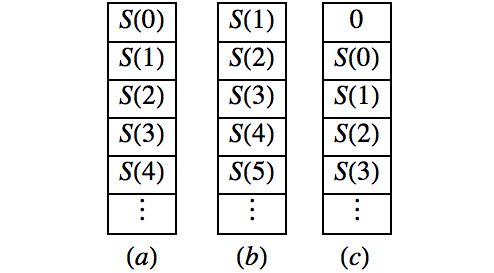
\includegraphics[width=1\linewidth]{images/fig-pop-push.png}
\caption{Stack interpretation of pop and push operation\label{fig-pop-push}}
\end{figure}
\begin{example}[Some Sequence Operations]\label{ex-some-sequence-operations}
If \(S(n) = n\), \(T(n) = n^2\), \(U(n) = 2^n\), and \(R(n) =n 2^n\) %
\par
\leavevmode%
\begin{enumerate}[label=\alph*]
\item\hypertarget{li-131}{} \((S + T)(n) = n + n^2\)%
\item\hypertarget{li-132}{}\((U + R)(n) = 2^n+ n 2^n= (1+n)2^n\)%
\item\hypertarget{li-133}{}\((2 U)(n) = 2\cdot 2^n= 2^{n+1}\)%
\item\hypertarget{li-134}{} \(\left(\frac{1}{2}R\right)(n)= \frac{1}{2}n 2^n= n 2^{n-1}\)%
\item\hypertarget{li-135}{} \((S\cdot T)(n) = n n^2 = n^3\)%
\item\hypertarget{li-136}{}\((S*T)(n)= \sum_{j=0}^n S(j) T(n-j)= \sum_{j=0}^n j (n-j)^2\\
\\
\quad \quad =\sum_{j=0}^n \left( j n^2-2 n j^2 + j^3\right)\\
\\
\quad \quad = n^2\sum_{j=0}^n j-2n \sum_{j=0}^n j^2 + \sum_{j=0}^n j ^3\\
\\
\quad \quad =n^{2 }\left(\frac{n (n+1)}{2}\right)- 2n\left(\frac{(2n+1)(n+1)n}{6}\right)+\frac{1}{4} n^2 (n+1)^2\\
\\
\quad \quad = \frac{n^2(n+1)(n-1)}{12}\)%
\item\hypertarget{li-137}{}\((U*U)(n) =\sum_{j=0}^n U(j) U(n-j)\\
\\
\quad \quad =\sum_{j=0}^n 2^j 2^{n-j}\\
\\
\quad \quad = (n+1)2^n\)%
\item\hypertarget{li-138}{} \((S\uparrow )(n)=n+1\)%
\item\hypertarget{li-139}{}\((S\downarrow )(n)=\max (0,n-1)\)%
\item\hypertarget{li-140}{} \(((S\downarrow )\downarrow )(n)= \max (0, n - 2)\)%
\item\hypertarget{li-141}{} \((U\downarrow )(n)=\left\{
\begin{array}{cc}
 2^{n-1} & \textrm{ if } n>0 \\
 0 & \textrm{ if } n=0 \\
\end{array}
\right.\)%
\item\hypertarget{li-142}{} \(((U\downarrow )\uparrow )(n)=(U\downarrow )(n+1)= 2^n= U(n)\)%
\item\hypertarget{li-143}{} \(((U\uparrow )\downarrow ) (n)=\left\{
\begin{array}{cc}
 0 & \textrm{ if } n = 0 \\
 U(n) & \textrm{ if } n>0 \\
\end{array}
\right.\)%
\end{enumerate}
%
\end{example}
\par
Note that \((U\downarrow )\uparrow \neq (U\uparrow )\downarrow\).%
\begin{definition}[ Multiple Pop and Push]\label{def-multiple-pop-and-push}
\index{Multiple Pop and Push:}\label{notation-6}
\label{notation-7}
If S is a sequence of numbers and \(p\) a positive integer greater than 1, define
\[S\uparrow p = (S\uparrow (p - 1))\uparrow\textrm{ if }p \geq  2 \textrm{ and }S\uparrow 1 = S\uparrow\] 
Similarly, define
\[S\downarrow p = (S\downarrow (p - 1))\downarrow\)\textrm{ if } p \geq  2\textrm{ and }S\downarrow 1 = S\downarrow\]
%
\end{definition}
\par
In general, \(S \uparrow p)(k) = S(k+p),\) and



\begin{equation*}
(S\downarrow p)(k)=\left\{
   \begin{array}{cc}
 0 & \textrm{ if } k < p \\
 S(k-p) & \textrm{ if } k\geq p \\
\end{array}
\right.
\end{equation*}
%
\typeout{************************************************}
\typeout{Subsection 1.5.4 Operations on Generating Functions}
\typeout{************************************************}
\subsection[Operations on Generating Functions]{Operations on Generating Functions}\label{sss-operations-on-generating-functions}
\index{Generating Functions!Operations on,}\begin{definition}[Operations on Generating Functions]\label{definition-16}
\index{Generating Functions!Operations on,}If  \(G(z)=\sum_{k=0}^{\infty} a_k z^k\) and \(H(z) =\sum_{k=0}^{\infty} b_k z^k\)
are generating functions and \(c\) is a real number, then the sum \(G + H\), scalar product \(c G\), product \(G H\), and monomial product \(z^p G\), \(p \geq  1\) are generating functions, where

\begin{gather}
(G + H)(z)=\sum_{k=0}^{\infty} \left(a_k+b_k\right) z^k\label{gf-sum}\\
[(c G)(z)=\sum_{k=0}^{\infty} c a_k z^k\label{gf-scalarmult}\\
(G H)(z) = \sum_{k=0}^{\infty} c z^k \textrm{ where } c_k= \sum_{j=0}^k a_jb_{k-j}\label{gf-product}\\
\left(z^p G\right)(z) = z^p\sum_{k=0}^{\infty} a_k z^k=\sum_{k=0}^{\infty} a_k z^{k+p} = \sum_{n=p}^{\infty} a_{n-p} z^n\label{gf-shift}
\end{gather}
%
\par
The last sum is obtained by substituting \(n - p\) for \(k\) in the previous sum.%
\end{definition}
\begin{example}[Some operations on generating functions]\label{ex-some-gf-operations}
If

\(D(z) =\sum_{k=0}^{\infty} kz^k\) and \(H(z) =\sum_{k=0}^{\infty} 2^k z^k\) 

then

\((D + H)(z) =\sum_{k=0}^{\infty} \left(k+2^k\right) z^k\) 

\((2H)(z)= \sum_{k=0}^{\infty} 2\cdot 2^kz^k =\sum_{k=0}^{\infty} 2^{k+1}z^k\)

 \((z D)(z) = z\sum_{k=0}^{\infty} kz^k= \sum_{k=0}^{\infty} kz^{k+1}= \sum_{k=1}^{\infty} (k-1)
z^k \quad = D(z)- \sum_{k=1}^{\infty} z^k\)

\((D H)(z)=\sum_{k=0}^{\infty} \left(\sum_{j=0}^k j 2^{k-j}\right)z^k\)

\((H H)(z)= \sum_{k=0}^{\infty} \left(\sum_{j=0}^k 2^j2^{k-j}\right) z^k=\sum_{k=0}^{\infty} (k+1)2^k z^k\)%
\par
Note: \(D(z) = G(S;z)\), and \(H(z) = G(U;z)\) from Example 8.5.2.%
\end{example}
Now we establish the connection between the operations on sequences and generating
functions. Let \(S\) and \(T\) be sequences and let \(c\) be a real number.

\begin{gather}
G(S+T;z)=G(S;z)+G(T;z)\label{gf-ops-1}\\
G(cS;z)=c G(S;z)\label{gf-ops-2}\\
 G(S*T;z)=G(S;z) G(T;z)\label{gf-ops-3}\\
 G(S\uparrow ;z)=(G(S;z)-S(0))/z\label{gf-ops-4}\\
 G(S\downarrow ;z)=z G(S;z)\label{gf-ops-5}
\end{gather}%
\par
In words, \hyperref[gf-ops-1]{(\ref{gf-ops-1})} says that the generating function of the sum of two sequences equals the sum of the generating functions of those sequences. Take
the time to write out the other four identities in your own words. From the previous examples, these identities should be fairly obvious, with the
possible exception of the last two. We will prove \hyperref[gf-ops-4]{(\ref{gf-ops-4})} as part of the next theorem and leave the proof of \hyperref[gf-ops-5]{(\ref{gf-ops-5})} to the interested reader. Note that
there is no operation on generating functions that is related to sequence multiplication; that is, \(G(S\cdot T;z)\) cannot be simplified.%
\begin{theorem}[Generating functions related to Pop and Push]\label{gf-of-pop-push}
If \(p > 1\),%
\par
\leavevmode%
\begin{enumerate}[label=\alph*]
\item\hypertarget{li-144}{}\(G(S\uparrow p;z) = \left(G(S;z) -\left.\sum_{k=0}^{p-1} S(k) z^k\right)/z^k\right.\)%
\item\hypertarget{li-145}{} \(G(S\downarrow p;z) = z^p G(S;z)\).%
\end{enumerate}
%
\end{theorem}
\begin{proof}\hypertarget{proof-2}{}
We prove (a)  by induction and leave the proof of (b) to the reader.  %
\par
Basis: 
\begin{equation*}
\begin{split}
  G(S\uparrow;z) &= \sum_{k=0}^{\infty} S(k+1) z^k\\
  		& =\sum_{k=1}^{\infty} S(k) z^{k-1}\\
  		& =\left.\left(\sum_{k=1}^{\infty} S(k) z^k\right)\right/z\\ 		
  		& =\left.\left(S(0)+\sum_{k=1}^{\infty} S(k) z^k-S(0)\right)\right/z\\
  		& =(G(S;z)-S(0))/z
\end{split}
\end{equation*}

Therefore, part (a) is true for \(p=1\).%
\par
Induction: Suppose that for some \(p\geq 1\), the statement in part (a) is true:

\begin{equation*}
\begin{split}
 G(S\uparrow (p+1);z) &= G((S\uparrow p)\uparrow ;z)\\
		& = (G(S\uparrow p ;z)-(S\uparrow p)(0))/z \textrm{ by the basis}\\
		& = \frac{\frac{\left(G(S;z)-\sum_{k=0}^{p-1} S(k) z^k\right)}{z^p}-S(p)}{z}
\end{split}
\end{equation*}

by the induction hypothesis. Now write \(S(p)\) in the last expression above as \(\left(S(r)z^p \right)/z^p\) so that it fits into the finite summation:

\begin{equation*}
\begin{split}
 G(S\uparrow (p+1);z) & =\left.\left(\frac{G(S;z)-\sum_{k=0}^p S(k) z^k}{z^p}\right)\right/z\\
					& = \left(G(S;z)-\sum_{k=0}^p S(k) z^k\right)/z^{p+1}
\end{split}
\end{equation*}
%
\par
Therefore the statement is true for \(p+1\).\(\square\)%
\end{proof}
\typeout{************************************************}
\typeout{Subsection 1.5.5 Closed Form Expressions for Generating Functions}
\typeout{************************************************}
\subsection[Closed Form Expressions for Generating Functions]{Closed Form Expressions for Generating Functions}\label{ss-closed-form-expressions-for-generating-functions}
\index{Generating Functions!Closed form expressions for}The most basic tool used to express generating functions in closed form is the closed form expression for the geometric series, which is an expression
of the form \(a + a r + a r^2+ \cdots\). It can either be terminated or extended infinitely.%
\par
Finite Geometric Series: 
\begin{gather}
a + a r + a r^2+ \cdots +a r^n= a\left(\frac{1-r^{n+1}}{1-r}\right)
\label{finite-geometric-series}
\end{gather} %
\par
Infinite Geometric Series:
\begin{gather}
a + a r + a r^2+ \cdots = \frac{a}{1-r}
\label{infinite-geometric-series}
\end{gather} %
\par
Restrictions: 
\(a\) and \(r\) represent constants and the right sides of the two equations apply under the following conditions:%
\par
\leavevmode%
\begin{enumerate}[label=\arabic*]
\item\hypertarget{li-146}{}\(r\) must not equal 1 in the finite case. Note that \(a + a r + \cdots  a r^n = (n + 1)a\) if\(r = 1\).%
\item\hypertarget{li-147}{} In the infinite case, the absolute value of \(r\) must be less than 1.%
\end{enumerate}
%
\par
These restrictions don't come into play with generating functions. We could derive \hyperref[finite-geometric-series]{(\ref{finite-geometric-series})} by noting that if \(S(n) = a + a r +\cdots  + a r^n\), \(n
> 0\), then \(S(n) = r S(n - 1) + a\) (See Exercise 10 of Section 8.3). An alternative derivation was used in Section 8.4. We will take the same
steps to derive \hyperref[infinite-geometric-series]{(\ref{infinite-geometric-series})}. Let \(x = a + a r + a r^2 + \cdots \).  Then

\begin{equation*}r x =a r+ ar^2 +\cdots = x- a \Rightarrow x-rx=a \Rightarrow x=  \frac{a}{1-r}\end{equation*}
%
\begin{example}[Generating Functions involving Geometric Sums]\label{ex-geometric-sums}
\leavevmode%
\begin{enumerate}[label=\alph*]
\item\hypertarget{li-148}{} If \(S(n) = 9\cdot 5^n\), \(n \geq  0\), \(G(S;z)\) is an infinite geometric series with \(a = 9\) and \(r = 5z\).Therefore,  \(G(S;z) = \frac{9}{1 - 5z}\).%
\item\hypertarget{li-149}{} If \(T(n) = 4\), \(n \geq\)0, then \(G(T;z) = 4/(1 - z)\).%
\item\hypertarget{li-150}{}If \(U(n) = 3(-1)^n\), then \(G(U;z) = 3/(1 + z)\).%
\item\hypertarget{li-151}{}Let \(C(n) = S(n) + T(n) + U(n) = 9 \cdot  5^n + 4 + 3(-1)^n\).  Then

\begin{equation*}
\begin{split}
G(C;z) & = G(S;z) + C(T;z) + G(U;z)\\
		& = \frac{9}{1-5z} + \frac{4}{1-z}+ \frac{3}{1+z}\\
		& = -\frac{14 z^2+34z-16}{5 z^3-z^2-5 z+1}
\end{split}
\end{equation*}%
\par
Given a choice between the last form of \(G(C;z)\) and the previous sum of three fractions, we would prefer leaving it as a sum of three functions.
As we saw in an earlier example, a partial fractions decomposition of a fraction such as the last expression requires some effort to produce.%
\item\hypertarget{li-152}{} If \(G(Q;z) = 34/(2 - 3z)\), then \(Q\) can be determined by multiplying the numerator and denominator by 1/2 to obtain \(\frac{17}{1-\frac{3}{2}z}\).
We recognize this fraction as the sum of the infinite geometric series with \(a = 17\) and \(r = \frac{3}{2}z\). Therefore \(Q(n) = 17(3/2)^n\).%
\item\hypertarget{li-153}{}If \(G(A;z) = (1 + z)^3\) , then we expand \((1 + z)^3\)to \(1 + 3z + 3z^2 + z^{3}\) . Therefore \(A(0) = 1\), \(A(1) = 3\) \(A(2)= 3\), \(A(3) = 1\), and, since there are no higher-powered terms, \(A(n) = 0\), \(n \geq  4\). A more concise way of describing \(A\) is \(A(k)
= C(3;k)\), since \(C(n,k)\) is interpreted as 0 of \(k > n\).
%
\end{enumerate}
%
\end{example}
\par
\hyperref[table-gf-closed-form]{Table~\ref{table-gf-closed-form}} lists some closed form expressions for the generating functions of some common sequences.%
\leavevmode%
\begin{table}
\centering
\begin{tabular}{cc}\hrulethick
\(\)&\(\)\tabularnewline[0pt]
 Sequence&Generating Function\tabularnewline[0pt]
\(S(k)=b a^k\)&\(G(S;z)=\frac{b}{1-a z}\)\tabularnewline[0pt]
\(S(k)=k\)&\(G(S;z)=\frac{z}{(1-z)^2}\)\tabularnewline[0pt]
\(S(k)=b k a^k\)&\(G(S;z)=\frac{a b z}{(1-a z)^2}\)\tabularnewline[0pt]
\(S(k) = \frac{1}{k!}\)&\(G(S;z)=e^z\)\tabularnewline[0pt]
\(S(k) = \left\{
\begin{array}{cc}
 C(n;k) & 0\leq k\leq n \\
 0 & k>n \\
\end{array}\right.\)&\( G(S;z)=(1+z)^n\)\tabularnewline[0pt]
\(\)&\(\)\tabularnewline[0pt]
\(\)&\(\)
\end{tabular}
\caption{Closed Form Expressions of some Generating Functions\label{table-gf-closed-form}}
\end{table}
\begin{example}[Another Complete Solution]\label{ex-another-complete-solution}
 Solve \(S(k) + 3S(k - 1) - 4S(k -2) = 0\), \(k\geq 2\), with \(S(0) = 3\) and \(S(1) = -2\). The solution will be derived using the same steps that were used earlier in this section, with one variation.%
\par
\leavevmode%
\begin{enumerate}[label=\arabic*]
\item\hypertarget{li-154}{}Translate to an equation about generating functions. First, we change the index of the recurrence relation by substituting \(n + 2\) for \(k\).
The result is \(S(n + 2) + 3S(n + 1) - 4S(n) = 0\), \(n \geq  0\).Now, if \(V(n) = S(n + 2) + 35 (n + 1) - 4S(n)\), then \(V\) is the zero
sequence, which has a zero generating function. Furthermore, \(V = S\uparrow 2+3(S\uparrow )-4 S\) . Therefore,

\(0 = G(V;z) \\
\\
\quad = G(S\uparrow 2; z) + 3 G(S\uparrow ;z) - 4G(S;z) \\
\\
\quad = \frac{G(S;z) - S(0) - S(1)z }{z^2}+4 \frac{(G(S;z) - S(0))}{z} - 4G(S;z)\).%
\item\hypertarget{li-155}{}We want to now solve the following equation for \(G(S;z)\):
 \(\frac{G(S;z) - S(0) - S(1)z }{z^2}+4 \frac{(G(S;z) - S(0))}{z} - 4G(S;z) = 0\)

Multiply by \(z^2\) :

\(G(S;z) - 3 + 2z + 3z(G(S;z) - 3) - 4z^2 G(S;z) = 0\)

Expand and collect all terms involving \(G(S;z)\) on one side of the equation:

\(G(S;z) + 3z G(S;z) - 4z^2 G(S;z) = 3 + 7z\) 

\(\left(1 + 3z - 4z^2 \right)G(S;z)= 3 + 7z\) 

Therefore,

\(G(S;z)= \frac{3+7z}{1 + 3z - 4z^2}\)%
\item\hypertarget{li-156}{} Determine S from its generating function.
 \(1 + 3z - 4z^2 = (1 + 4z) (1 - z)\)
thus a partial fraction decomposition of \(G(S;z)\) would be:

\(\frac{A}{1+4z}+ \frac{B}{1-z}=\frac{A z-A-4 B z-B}{(z-1) (4 z+1)}\\
\\
\quad \quad =\frac{(A+B)+(4B-A)z}{(z-1) (4 z+1)}\)

Therefore, \(A + B = 3\) and \(4B - A = 7\). The solution of this set of equations is \(A = 1\) and \(B = 2\).

\(G(S;z)= \frac{1}{1+4z}+ \frac{2}{1-z}\)

\(\frac{1}{1+4z}\) is the generating function of \(S_1(n)=(-4)^n\), and

\(\frac{2}{1-z}\) is the generating function of \(S_2(n) = 2(1)^n = 2\).

In conclusion, since \(G(S;z) = G\left(S_1;z\right) + G\left(S _2;z\right)\), \(S(n) = 2 + (-4)^n\).
%
\end{enumerate}
%
\end{example}
\begin{example}[An Application to Counting]\label{example-counting-application}
 Let \(A = \{a, b, c, d, e\}\) and let \(A^*\) be the set of all strings of length zero or more that can be made using each of the elements of \(A\) zero or more times. By the generalized rule of products, there are \(5^n\) such strings that have length \textit{
n}, \(n\geq 0\), Suppose that \(X_n\) is the set of strings of length \(n\) with the property that all of the \(a\)'s and \textit{ b'}s precede all of the \(c\)'s, \(d\)'s, and \(e\)'s. Thus \(\text{aaabde} \in  X_6\), but \(\text{abcabc} \notin  X_6\). Let \(R(n)
=\left|X_n\right|\).A closed form expression for \(R\) can be obtained by recognizing \(R\) as the convolution of two sequences.
To illustrate our point, we will consider the calculation of \(R(6)\).%
\par
Note that if a string belongs to \(X_6\), it starts with \(k\) characters from \(\{a, b\}\) and is followed by \(6 - k\) characters from \(\{c,
d, e\}\). Let \(S(k)\) be the number of strings of \(a\)'s and \(b\)'s with length \(k\) and let \(T(k)\) be the number of strings
of \(c\)'s, \(d\)'s, and \(e\)'s with length \(k\). By the generalized rule of products, \(S(k) = 2^k\) and \(T(k) = 3^k\).
Among the strings in \(X_6\) are the ones that start with two \(a\)'s and \(b\)'s and end with \(c\)'s, \(d\)'s, and \textit{
e}'s. There are \(S(2)T(4)\) such strings. By the law of addition, \(\left.\left|X_6\right| =R(6)=S(0)T(6)+S(1)T(5)+\cdots +S(5)T(1)+S(6)T(0\right)\).
Note that the sixth term of R is the sixth term of the convolution of \(S\) with \(T\), \(S*T\). Think about the general situation for
a while and it should be clear that \(R =S*T\). Now, our course of action will be to:%
\par
\leavevmode%
\begin{enumerate}[label=\alph*]
\item\hypertarget{li-157}{}Determine the generating functions of \(S\) and \(T\),%
\item\hypertarget{li-158}{}Multiply \(G(S;z)\) and\(G(T;z)\) to obtain \(G(S*T;z) = G(R;z)\) (by 10.5e), and%
\item\hypertarget{li-159}{}Determine \(R\) on the basis of\(G(R;z)\).%
\end{enumerate}
%
\par
\leavevmode%
\begin{enumerate}[label=\alph*]
\item\hypertarget{li-160}{}\(G(S;z) =\sum_{k=0}^{\infty} 2^k z^k=\frac{1}{1-2z}\) , and \(G(T;z) =\sum_{k=0}^{\infty} 3^k z^k=\frac{1}{1-3z}\)%
\item\hypertarget{li-161}{} \(G(R;z) = G(S;z)G(T;z) = \frac{1}{(1-2z)(1-3z)}\)%
\item\hypertarget{li-162}{}To recognize \(R\) from \(G(R;z)\), we must do a partial fractions decomposition:



 \(\frac{1}{(1-2z)(1-3z)}=\frac{A}{1-2z}+\frac{B}{1-3z}=\frac{-3 A z+A-2 B z+B}{(2 z-1) (3 z-1)}=\frac{(A+B)+(-3 A -2 B )z}{(2 z-1) (3 z-1)}\)

Therefore, \(A + B = 1\) and \(-3A - 2B = 0\). The solution of this pair of equations is \(A = - 2\) and \(B = 3\).

Since



 \(G(R;z) =\frac{-2}{1-2z}+\frac{3}{1-3z}\),

which is the sum of the generating functions of \(-2(2)^k\) and \(3 (3)^k\),

\(R(k) =-2(2)^k+3 (3)^k = 3^{k+1}-2^{k+1}\) %
\par
For example, \(R(6) = 3^7 - 2^7= 2187 - 128 = 2059\). Naturally, this equals the sum that we get from \((S*T)(6)\).To put this number
in perspective, the total number of strings of length 6 with no restrictions is \(5^6=15625\), and \(\frac{2059}{15625}\approx 0.131776\).Therefore
approximately 13 percent of the strings of length 6 satisfy the conditions of the problem.

%
\end{enumerate}
%
\end{example}
\typeout{************************************************}
\typeout{Subsection 1.5.6 Extra for Experts}
\typeout{************************************************}
\subsection[Extra for Experts]{Extra for Experts}\label{ss-extra-for-experts}
The remainder of this section is intended for readers who have had, or who intend to take, a course in combinatorics. We do not advise that it be
included in a typical course. The method that was used in \hyperref[example-counting-application]{Example~\ref{example-counting-application}} is a very powerful one and can be used to solve many problems in combinatorics.
We close this section with a general description of the problems that can be solved in this way, followed by some examples.%
\par
Consider the situation in which \(P_1\), \(P_2\), \(\ldots\), \(P_m\) are \(m\) actions that must be taken, each of which results in a well-defined
outcome. For each\(k = 1,2, . . . ,m\) define \(X_k\) to be the set of possible outcomes of \(P_k\) . We will assume that each outcome can be quantified
in some way and that the quantification of the elements of \(X_k\) is defined by the function \(Q_k : X_k \to  \{0, 1,2, . . .\}\). Thus, each outcome
has a non-negative integer associated with it. Finally, define a frequency function \(F_k : \{0, 1, 2, . . .\} \to  \{0, 1, 2, . . .\}\) such that
\(F_k(n)\) is the number of elements of \(X_k\) that have a quantification of \(n\).%
\par
Now, based on these assumptions, we can define the problems that can be solved. If a process \(P\) is defined as a sequence of actions \(P_1,P_2,\ldots
,P_m\) as above, and if the outcome of \(P\), which would be an element of \(X_1\times X_2\times \cdots \times X_m\), is quantified by

 \[Q\left(a_1,a_2, \ldots , a_m\right)= \sum_{k=1}^m Q_k\left(a_k\right)\]



then the frequency function, \(F\), for \(P\) is the convolution of the frequency functions for\(P_1\), \(P_2\), \(\ldots\), \(P_m\),
which has a generating function equal to the product of the generating functions of the frequency functions \(F_1\), \(F_2\), \(\ldots\), \(F_m\).  That is,

\begin{equation*}
G(F;z) =G\left(F_1;z\right)G\left(F_2;z\right) \cdots \left(F_m;z\right)
\end{equation*}

%
\begin{example}[Rolling Two Dice]\label{ex-dice-roll}
 Suppose that you roll a die two times and add up the numbers on the top face for each roll. Since the faces on the die represent
the integers 1 through 6, the sum must be between 2 and 12. How many ways can any one of these sums be obtained? Obviously, 2 can be obtained only
one way, with two 1's. There are two sequences that yield a sum of 3: 1-2 and 2-1. To obtain all of the frequencies with which the numbers 2 through
12 can be obtained, we set up the situation as follows. For \(j = 1, 2\);\(P_j\) is the rolling of the die for the \(j^{\text{th}}\) time. \(X_j
= \{1, 2, . . . , 6\}\) and \(Q_j : X_j \rightarrow \{0, 1, 2, 3,\ldots \}\) is defined by \(Q_j(x) = x\). Since each number appears on a die exactly once,
the frequency function is \(F_j(k)=1\) if \(1 \leq  k \leq  6\), and \(F_j(k) = 0\) otherwise. The process of rolling the die two times is quantified
by adding up the \(Q_j's\); that is, \(Q\left(a_1, a_2\right) =Q_{1}\left(a_1\right)+Q_2\left(a_2\right)\) . The generating function for the
frequency function of rolling the die two times is then

\begin{equation*}
\begin{split}
G(F; z) & = G\left(F_1;z\right)G\left(F_2;z\right)\\
		&  = (z^6+z^5+z^4+z^3+z^2+z)^2\\
		& =z^{12}+2 z^{11}+3 z^{10}+4 z^9+5 z^8+6 z^7+5 z^6+4 z^5+3 z^4+2
z^3+z^2
\end{split}
\end{equation*}
%
\par
Now, to get \(F(k)\), just read the coefficient of \(z^k\).For example, the coefficient of \(z^5\) is 4, so there are four ways to roll a total
of 5.%
\par
To apply this method, the crucial step is to decompose a large process in the proper way so that it fits into the general situation that we've described.
%
\end{example}
\begin{example}[Distribution of a Committee]\label{ex-committee-distribution}
Suppose that an organization is divided into three geographic sections, A, B, and C. Suppose that an executive committee of
11 members must be selected so that no more than 5 members from any one section are on the committee and that Sections A, B, and C must have minimums
of 3, 2, and 2 members, respectively, on the committee. Looking only at the number of members from each section on the committee, how many ways can
the committee be made up? One example of a valid committee would be 4 A's, 4 B's, and 3 C's.



Let \(P_A\) be the action of deciding how many members (not who) from Section A will serve on the committee. \(X_A= \{3, 4, 5\}\) and \(Q_A(k)=k\).
{ }The frequency function, \(F_A\) , is defined by \(F_A(k)=1\) if \(k\in X_k\) , with \(F_A(k)=0\) otherwise. \(G\left(F_A;z\right)\) is then \(z^3+
z^4+z^5\) . Similarly, \(G\left(F_B;z\right) =z^2+ z^3+ z ^4 + z^5= G\left(F_C ;z\right)\). Since the committee must have 11 members, our answer
will be the coefficient of \(z^{11}\) in \(G\left(F_A;z\right)G\left(F_B;z\right)G\left(F_C;z\right)\), which is 10:



\(G\left(F_A;z\right)G\left(F_B;z\right)G\left(F_C;z\right)=\left(z^3+ z^4+z^5\right)\left(z^2+ z^3+ z ^4 + z^5\right)^2\\
\\
\quad =z^{15}+3 z^{14}+6 z^{13}+9 z^{12}+10 z^{11}+9 z^{10}+6 z^9+3 z^8+z^7\)%
\end{example}
\typeout{************************************************}
\typeout{Exercises 1.5.7 Exercises for Section 8.5}
\typeout{************************************************}
\subsection[Exercises for Section 8.5]{Exercises for Section 8.5}\label{exercises-5}
\hypertarget{exercisegroup-10}{}\typeout{************************************************}
\typeout{Introduction  }
\typeout{************************************************}
A Exercises%
\begin{exercisegroup}
\item[1.]\hypertarget{exercise-37}{}What sequences have the following generating functions?%
\par
\leavevmode%
\begin{enumerate}[label=\alph*]
\item\hypertarget{li-163}{} 1%
\item\hypertarget{li-164}{}\(\frac{10}{2-z}\)%
\item\hypertarget{li-165}{} \(1 + z\)%
\item\hypertarget{li-166}{} \(\frac{3}{1+2z}+ \frac{3}{1-3z}\)%
\end{enumerate}
%
\par\smallskip
\par\smallskip
\noindent\textbf{Answer.}\hypertarget{answer-19}{}\quad
\leavevmode%
\begin{enumerate}[label=\alph*]
\item\hypertarget{li-167}{} \(1,0,0,0,0,\ldots\)%
\item\hypertarget{li-168}{} \(5(1/2)^k\) %
\item\hypertarget{li-169}{} \(1,1,0,0,0,\ldots\)%
\item\hypertarget{li-170}{} \(3(-2)^k+3\cdot 3^k\)%
\end{enumerate}
%
\item[2.]\hypertarget{exercise-38}{}What sequences have the following generating functions?%
\par
\leavevmode%
\begin{enumerate}[label=\alph*]
\item\hypertarget{li-171}{}\(\frac{1}{1+z}\)%
\item\hypertarget{li-172}{} \(\frac{1}{4-3z}\)%
\item\hypertarget{li-173}{}\(\frac{2}{1-z}+ \frac{1}{1+z}\)%
\item\hypertarget{li-174}{}\(\frac{z+2}{z+3}\)%
\end{enumerate}
%
\par\smallskip
\end{exercisegroup}
\par\smallskip\noindent
\hypertarget{exercisegroup-11}{}\typeout{************************************************}
\typeout{Introduction  }
\typeout{************************************************}
B Exercises%
\begin{exercisegroup}
\item[3.]\hypertarget{exercise-39}{}Find closed form expressions for the generating functions of the following sequences:%
\par
\leavevmode%
\begin{enumerate}[label=\alph*]
\item\hypertarget{li-175}{}\(V(n) = 9^n\)%
\item\hypertarget{li-176}{}\(P\), where \(P(k) - 6 P(k - 1) + 5 P(k - 2) = 0\) for \(k \geq  2\), with\(P(0) = 2\)and \(P(1) = 2\).%
\item\hypertarget{li-177}{} The Fibonacci sequence: \(F(k + 2) = F(k + 1) + F(k)\), \(k \geq  0\), with \(F(0) = F(1) = 1\).%
\end{enumerate}
%
\par\smallskip
\par\smallskip
\noindent\textbf{Answer.}\hypertarget{answer-20}{}\quad
\leavevmode%
\begin{enumerate}[label=\alph*]
\item\hypertarget{li-178}{} \(1/(1-9z)\) %
\item\hypertarget{li-179}{} \((2-10z)\left/\left(1-6z+5z^2\right)\right.\)%
\item\hypertarget{li-180}{} \(1\left/\left(1-z-z^2\right)\right.\)%
\end{enumerate}
%
\item[4.]\hypertarget{exercise-40}{}Find closed form expressions for the generating functions of the following sequences:%
\par
\leavevmode%
\begin{enumerate}[label=\alph*]
\item\hypertarget{li-181}{} \(W(n) = C(5;n)2^n\) for \(0 \leq  n \leq  5\) and \(W(n) = 0\) for \(n > 5\).%
\item\hypertarget{li-182}{} \(Q\), where \(Q(k) + Q(k - 1) - 42Q(k - 2) = 0\) for \(k\geq 2\), with \(Q(0) = 2\) and\(Q(1) = 2\).%
\item\hypertarget{li-183}{} \(G\), where \(G(k + 3) = G(k + 2) + G(k + 1) + G(k)\) for \(k \geq  0\), with \(G(0) = G(1) = G(2) = 1\).%
\end{enumerate}
%
\par\smallskip
\item[5.]\hypertarget{exercise-41}{}For each of the following expressions, find the partial fraction decomposition and identify the sequence having the expression as a generating
function.%
\par
\leavevmode%
\begin{enumerate}[label=\alph*]
\item\hypertarget{li-184}{} \(\frac{5+2z}{1-4z^2}\)%
\item\hypertarget{li-185}{} \(\frac{32-22z}{2-3z+z^2}\)%
\item\hypertarget{li-186}{} \(\frac{6-29z}{1-11z+ 30z^2}\)%
\end{enumerate}
%
\par\smallskip
\par\smallskip
\noindent\textbf{Answer.}\hypertarget{answer-21}{}\quad
\leavevmode%
\begin{enumerate}[label=\alph*]
\item\hypertarget{li-187}{} \(3/(1-2z)+2/(1+2z), 3\cdot 2^k+2(-2)^k\)%
\item\hypertarget{li-188}{} \(10/(1-z)+12/(2-z), 10+6(1/2)^k\)%
\item\hypertarget{li-189}{} \(-1/(1-5z)+7/(1-6z), 7\cdot 6^k-5^k\)%
\end{enumerate}
%
\item[6.]\hypertarget{exercise-42}{}Find the partial fraction decompositions and identify the sequence having the following expressions:%
\par
\leavevmode%
\begin{enumerate}[label=\alph*]
\item\hypertarget{li-190}{} \(\frac{1}{1-9z^2}\)%
\item\hypertarget{li-191}{} \(\frac{1+3z}{16-8z+z^2}\)%
\item\hypertarget{li-192}{} \(\frac{2z}{1-6z-7z^2}\)%
\end{enumerate}
%
\par\smallskip
\item[7.]\hypertarget{exercise-43}{} Given that \(S(k) = k\) and \(T(k) = 10k\), what is the \(k^{\text{th}}\) term of the generating function of each of the following sequences:%
\par
\leavevmode%
\begin{enumerate}[label=\alph*]
\item\hypertarget{li-193}{}\(S + T\)%
\item\hypertarget{li-194}{}\(S\uparrow  * T\) %
\item\hypertarget{li-195}{} \(S * T\)%
\item\hypertarget{li-196}{} \(S\uparrow *S\uparrow\)%
\end{enumerate}
%
\par\smallskip
\par\smallskip
\noindent\textbf{Answer.}\hypertarget{answer-22}{}\quad
\leavevmode%
\begin{enumerate}[label=\alph*]
\item\hypertarget{li-197}{} \(11k\)%
\item\hypertarget{li-198}{} \((5/3)k(k+1)(2k+1)+5k(k+1)\)%
\item\hypertarget{li-199}{} \(\underset{j=0}{\overset{k}{\Sigma }}(j)(10(k-j))=10k\underset{j=0}{\overset{k}{\Sigma }}j-10\underset{j=0}{\overset{k}{\Sigma }}j^2\)
    \(=5k^2(k+1)-(5k(k+1)(2k+1)/6)
=(5/3)k(k+1)(2k+1)\)%
\item\hypertarget{li-200}{} \(k(k+1)(2k+7)/12\)%
\end{enumerate}
%
\item[8.]\hypertarget{exercise-44}{}Given that \(P(k) = C(10;k)\) and \(Q(k) = k!\), what is the \(k^{\text{th}}\) term of the generating function of each of the following sequences:%
\par
\leavevmode%
\begin{enumerate}[label=\alph*]
\item\hypertarget{li-201}{}\(P * P\)%
\item\hypertarget{li-202}{}\(P + P\uparrow\)%
\item\hypertarget{li-203}{}\(P * Q\)%
\item\hypertarget{li-204}{} \(Q * Q\)%
\end{enumerate}
%
\par\smallskip
\end{exercisegroup}
\par\smallskip\noindent
\hypertarget{exercisegroup-12}{}\typeout{************************************************}
\typeout{Introduction  }
\typeout{************************************************}
C Exercises%
\begin{exercisegroup}
\item[9.]\hypertarget{exercise-45}{}A game is played by rolling a die five times. For the \(k^{\text{th}}\) roll, one point is added to your score if you roll a number higher
than \(k\). Otherwise, your score is zero for that roll. For example, the sequence of rolls \(2,3,4,1,2\) gives you a total score of three;
while a sequence of 1,2,3,4,5 gives you a score of zero. Of the \(6^5 = 7776\) possible sequences of rolls, how many give you a score of zero?, of
one? \(\ldots \) of five?%
\par\smallskip
\par\smallskip
\noindent\textbf{Answer.}\hypertarget{answer-23}{}\quad
 Coefficients of \(z^0\) through \(z^5\) in \((1+5z)(2+4z)(3+3z)(4+2z)(5+z)\)%
\par

\(\begin{array}{cc}
 k & \textrm{ Number of ways of getting a score of } k \\
 0 & 120 \\
 1 & 1044 \\
 2 & 2724 \\
 3 & 2724 \\
 4 & 1044 \\
 5 & 120 \\
\end{array}\)%
\item[10.]\hypertarget{exercise-46}{} Suppose that you roll a die ten times in a row and record the square of each number that you roll. How many ways could the sum of the squares
of your rolls equal 40? What is the most common outcome?%
\par\smallskip
\end{exercisegroup}
\par\smallskip\noindent
%
\backmatter
%
%
%% A lineskip in table of contents as transition to appendices, backmatter
\addtocontents{toc}{\vspace{\normalbaselineskip}}
%
\typeout{************************************************}
\typeout{References  References}
\typeout{************************************************}
\chapter[References]{References}\label{references-1}
%% If this is a top-level references
%%   you can replace with "thebibliography" environment
\begin{referencelist}
\bibitem[1]{biblio-sopowit-1983}\hypertarget{biblio-sopowit-1983}{}Sopowit, K. J., E. M. Reingold, and D. A. Plaisted \textit{The Traveling Salesman Problem and Minimum Matching in the Unit Square}.SIAM J. Computing, 1983,\textbf{12}, 144\textendash{}56.
\end{referencelist}
%
%% The index is here, setup is all in preamble
\printindex
%
\end{document}